\chapter{การทดลอง}
\label{chapter:result}

\section{การแบ่งข้อมูล}
ในการทดลองจะแบ่งข้อมูลออกเป็น 3 ชุด คือ ชุดข้อมูลสำหรับการเรียนรู้ (Training Set), ชุดข้อมูลสำหรับการตรวจสอบ (Validation Set) และชุดข้อมูลสำหรับการทดสอบ (Testing Set) โดยในแต่ละชุดข้อมูลจะมีความไม่สมดุลกันระหว่างกลุ่มข้อมูลส่วนมากและส่วนน้อย สำหรับ Training Set กับ Validation Set จะถูกใช้ในกระบวนการเรียนรู้ของโมเดล และ Testing Set จะถูกใช้ในการทดสอบโมเดลที่เรียนรู้มาแล้ว

\section{ชุดข้อมูล}

ในงานวิจัยนี้การทดลองถูกแบ่งออกเป็น 2 ส่วนหลัก ๆ คือ การทดลองกับชุดข้อมูลที่ไม่สมดุลสำหรับการวัดเปรียบเทียบสมรรถนะเกณฑ์มาตรฐาน (Benchmark) ตามที่ถูกนำเสนอไปใน~\cite{Ding:2011} และการทดลองกับชุดข้อมูลดัดแปลง โดยชุดข้อมูล CIFAR-100~\cite{Krizhevsky:2009} จะถูกดัดแปลงให้ไม่สมดุล สำหรับรายละเอียดการดัดแปลงนั้นจะถูกอธิบายไว้ในหัวข้อที่~\ref{ex:modified_dataset}

\subsection{ชุดข้อมูลดัดแปลง} \label{ex:modified_dataset}
การทดลองใน~\cite{Wang:2016} ได้ทำการดัดแปลง CIFAR-100 โดยการแบ่งชุดข้อมูลออกเป็น 3 ชุดข้อมูลย่อย คือ \emph{Tree1}, \emph{Tree2} และ \emph{Household} และเลือกข้อมูลมา 2 กลุ่มที่แตกต่างกันสำหรับแต่ละชุดข้อมูลย่อย ที่ซึ่งข้อมูลในแต่ละชุดข้อมูลย่อยจะถูกทำให้ไม่สมดุลกัน สำหรับรายละเอียดของกลุ่มข้อมูลในแต่ละชุดข้อมูลย่อยดังนี้

\paragraph{\emph{Tree1}}
เป็นชุดข้อมูลที่ประกอบด้วยข้อมูลของกลุ่ม maple tree และ oak tree โดยจะให้กลุ่ม maple tree เป็นกลุ่มข้อมูลส่วนมาก และ oak tree เป็นกลุ่มข้อมูลส่วนน้อย

\paragraph{\emph{Tree2}}
เป็นชุดข้อมูลที่ประกอบด้วยข้อมูลของกลุ่ม maple tree และ palm tree โดยจะให้กลุ่ม maple tree เป็นกลุ่มข้อมูลส่วนมาก และ palm tree เป็นกลุ่มข้อมูลส่วนน้อย

\paragraph{\emph{Household}}
เป็นชุดข้อมูลที่ประกอบด้วยข้อมูลของกลุ่ม household furniture และ household electrical devices โดยจะให้กลุ่ม household furniture เป็นกลุ่มข้อมูลส่วนมาก และ household electrical devices เป็นกลุ่มข้อมูลส่วนน้อย
\newline

แต่ละชุดข้อมูลย่อยจะถูกแบ่งออกเป็น 3 ชุด ก็คือ ชุดข้อมูลที่มีจำนวนตัวอย่างของกลุ่มข้อมูลส่วนน้อยเป็นร้อยละ 20, 10 และ 5 ของจำนวนตัวอย่างของกลุ่มข้อมูลส่วนมากตามลำดับ โดยจำนวนตัวอย่างของกลุ่มข้อมูลส่วนมากและส่วนน้อยใน Training Set ของแต่ละชุดข้อมูลแสดงดังรูปที่~\ref{fig:dist-cifar100}

\begin{figure}[h]
  \centering
  \subfigure[]{
      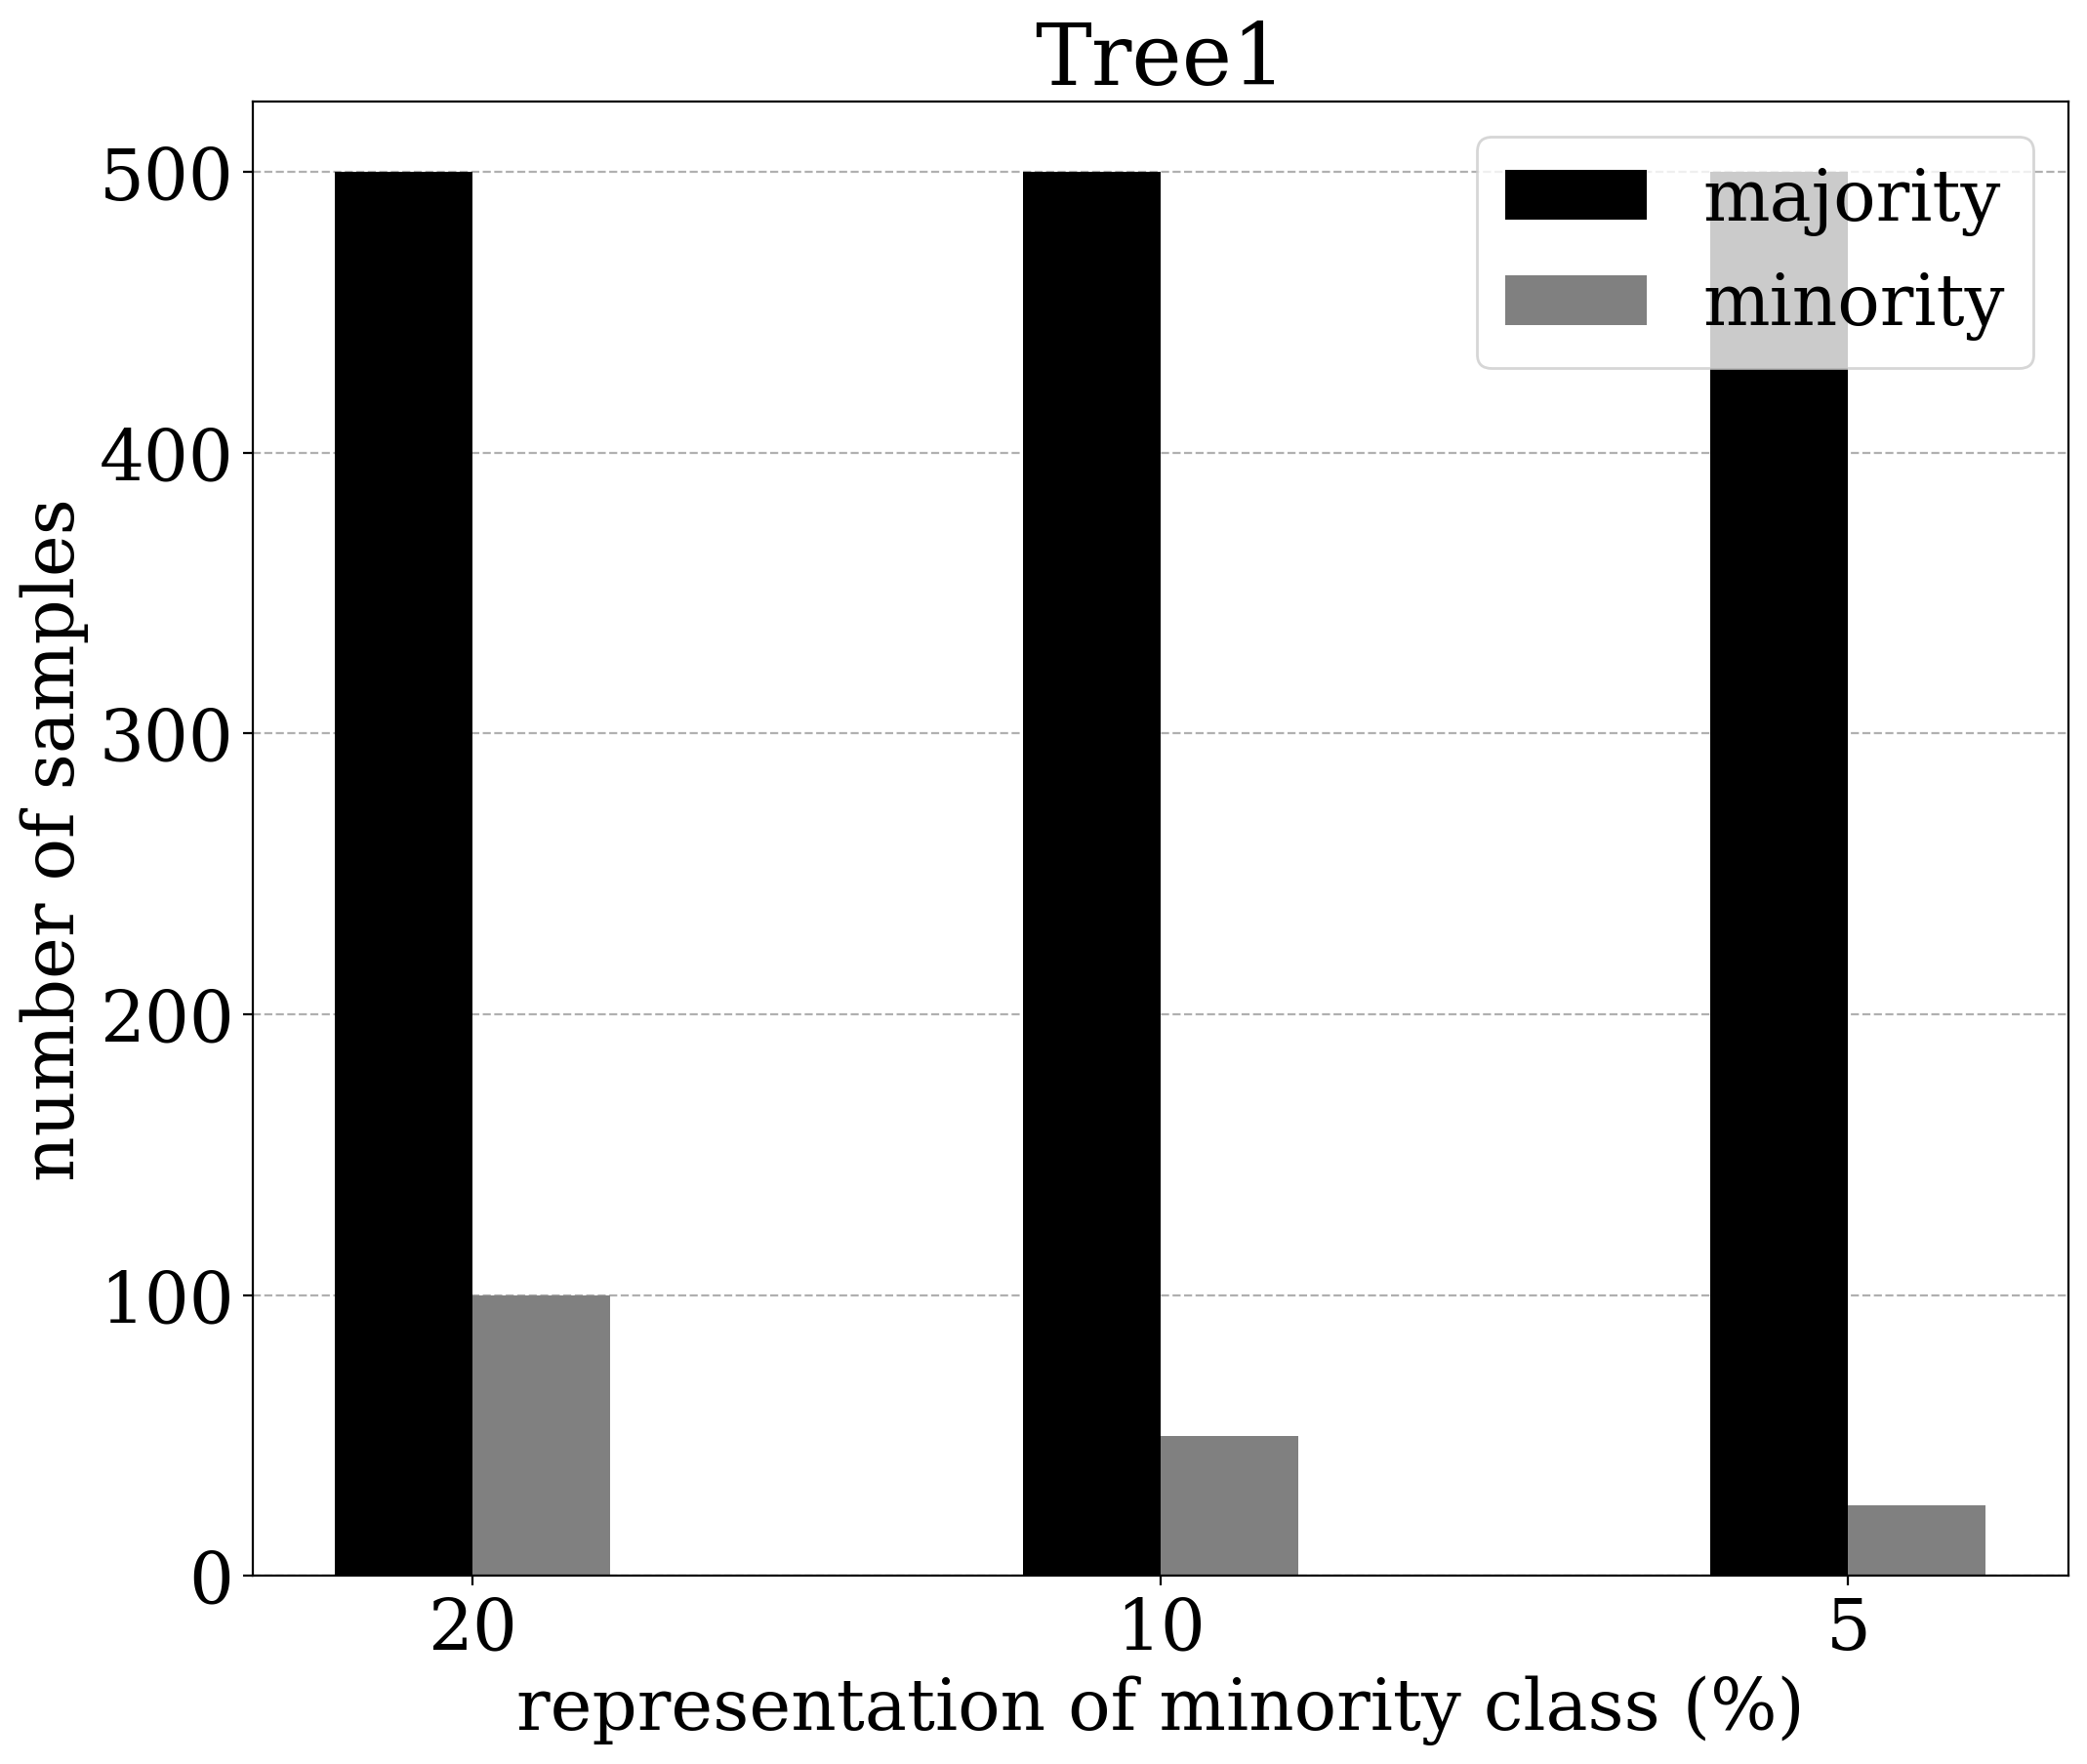
\includegraphics[width=0.45\columnwidth]{dataset/class_dist_Tree1_cifar100.png}
      \label{fig:dist-cifar100-tree1}
  }
  \subfigure[]{
    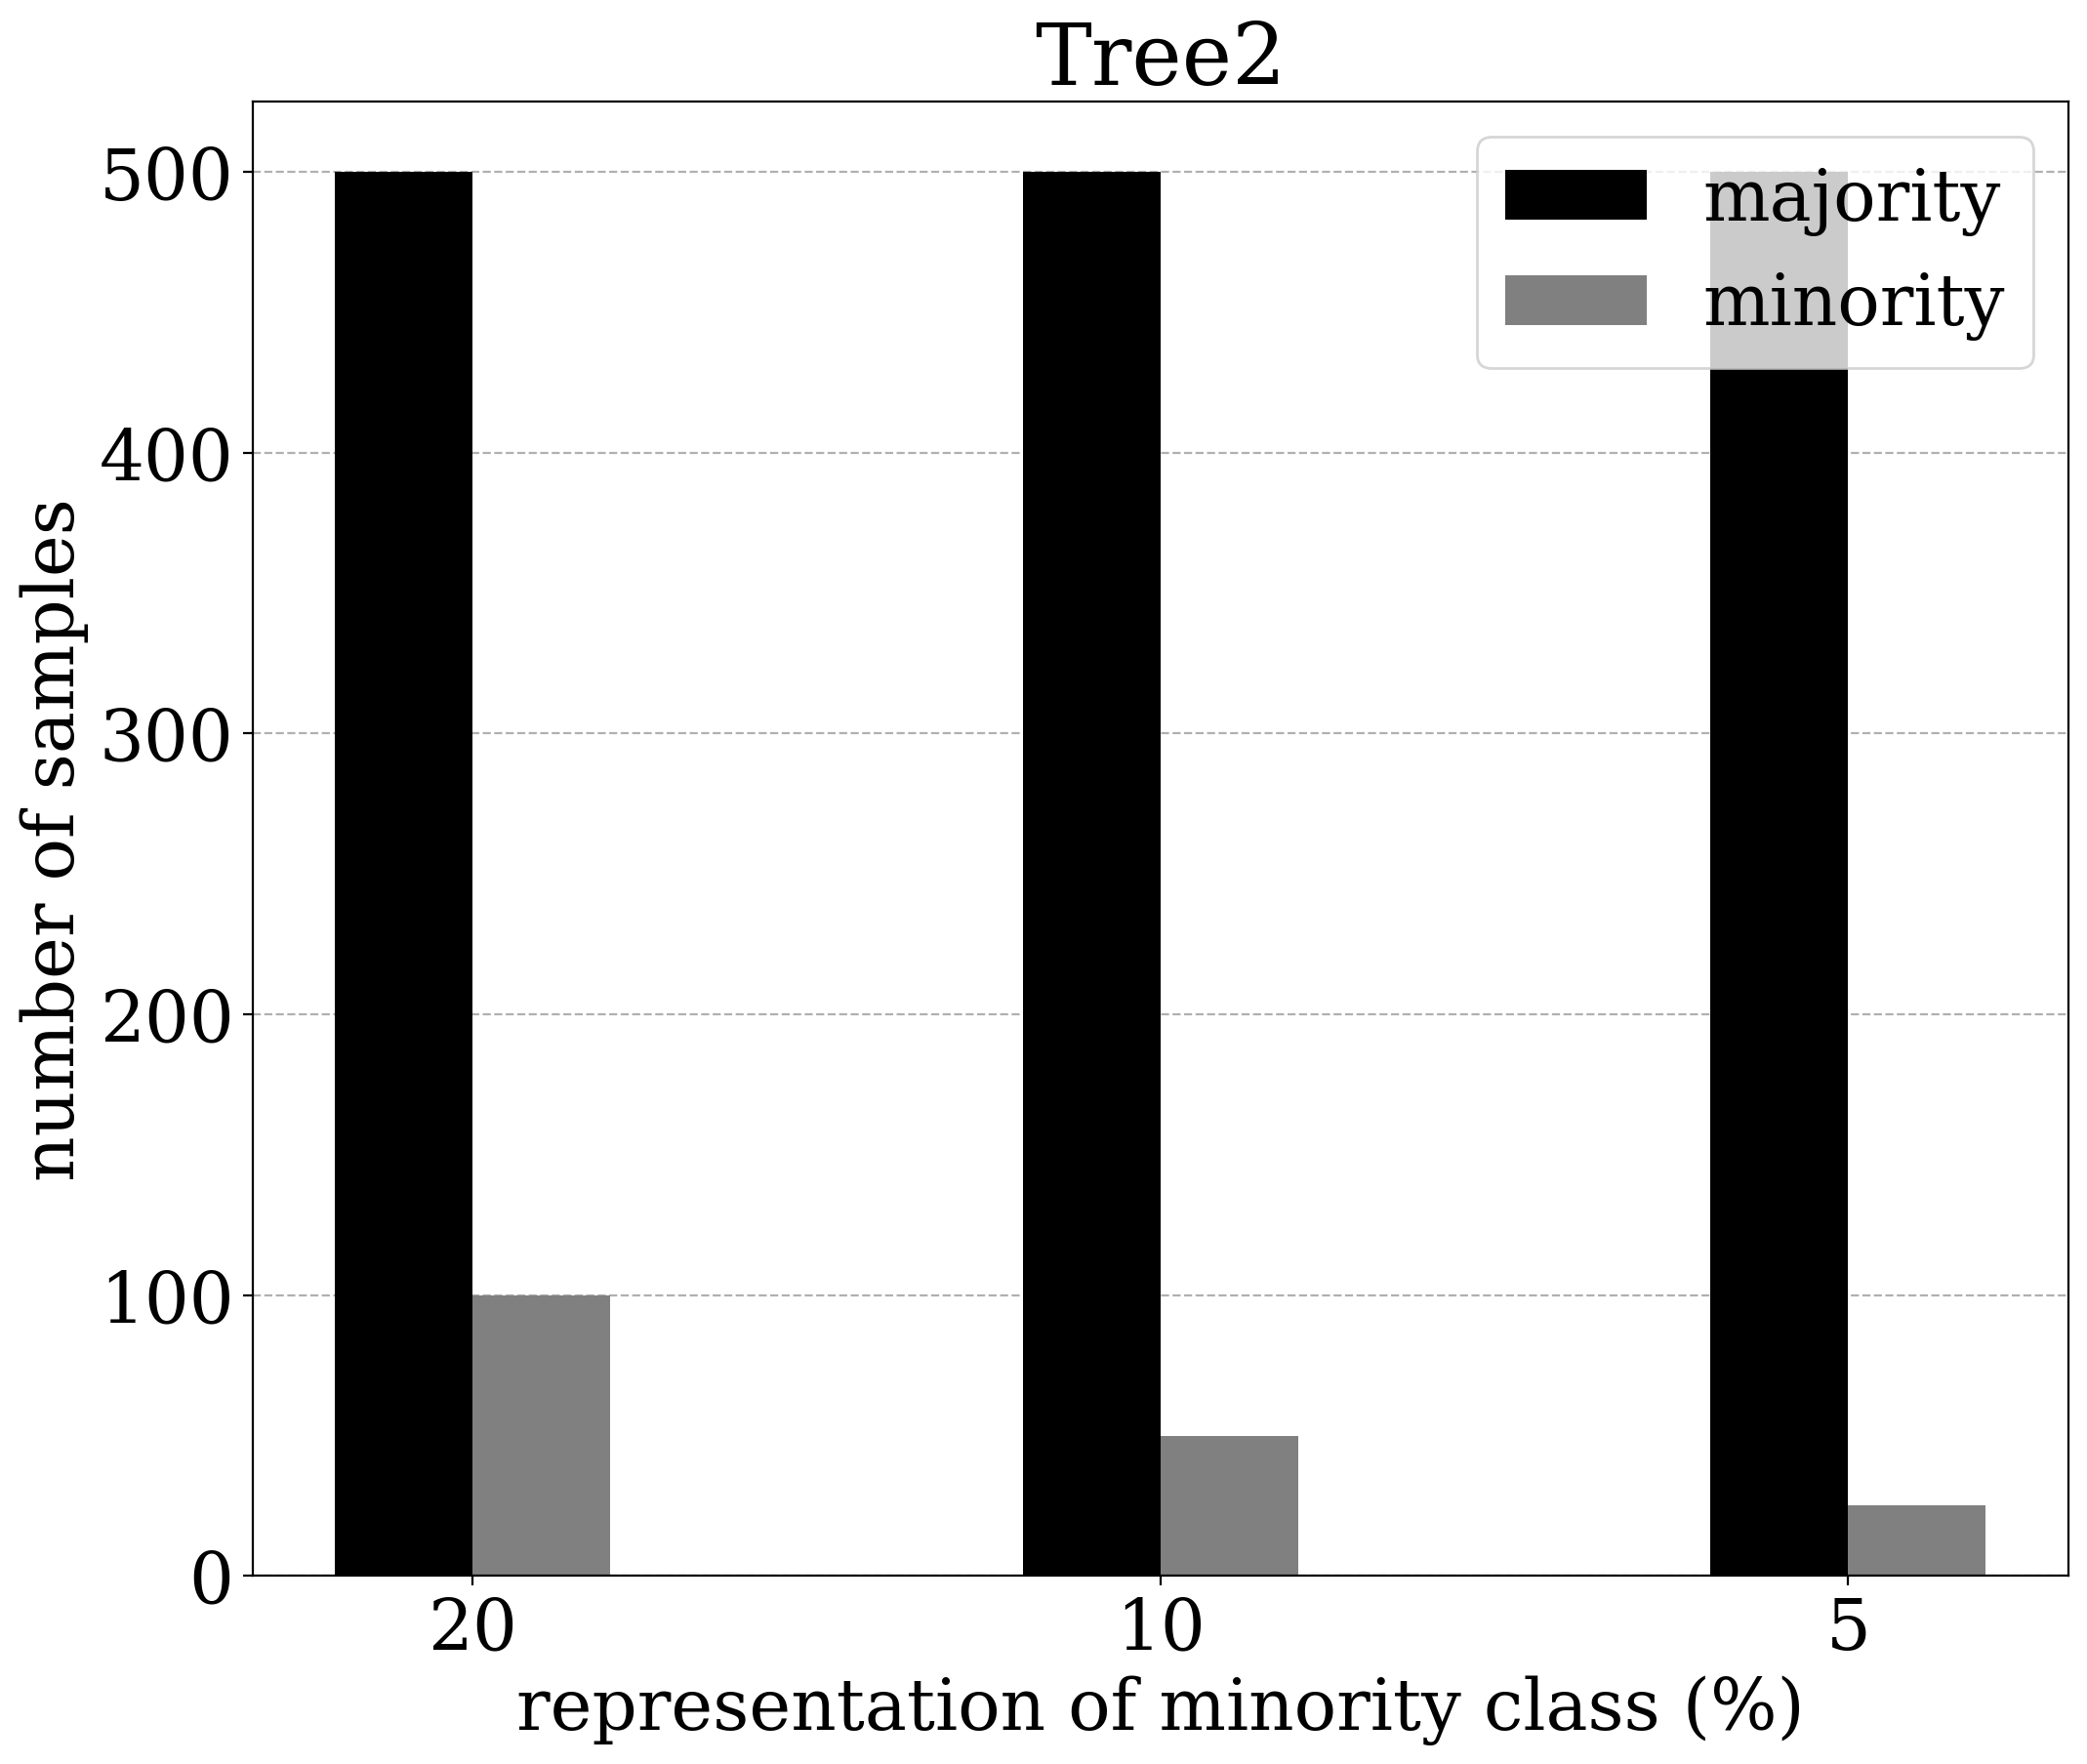
\includegraphics[width=0.45\columnwidth]{dataset/class_dist_Tree2_cifar100.png}
    \label{fig:dist-cifar100-tree2}
  }
   \subfigure[]{
      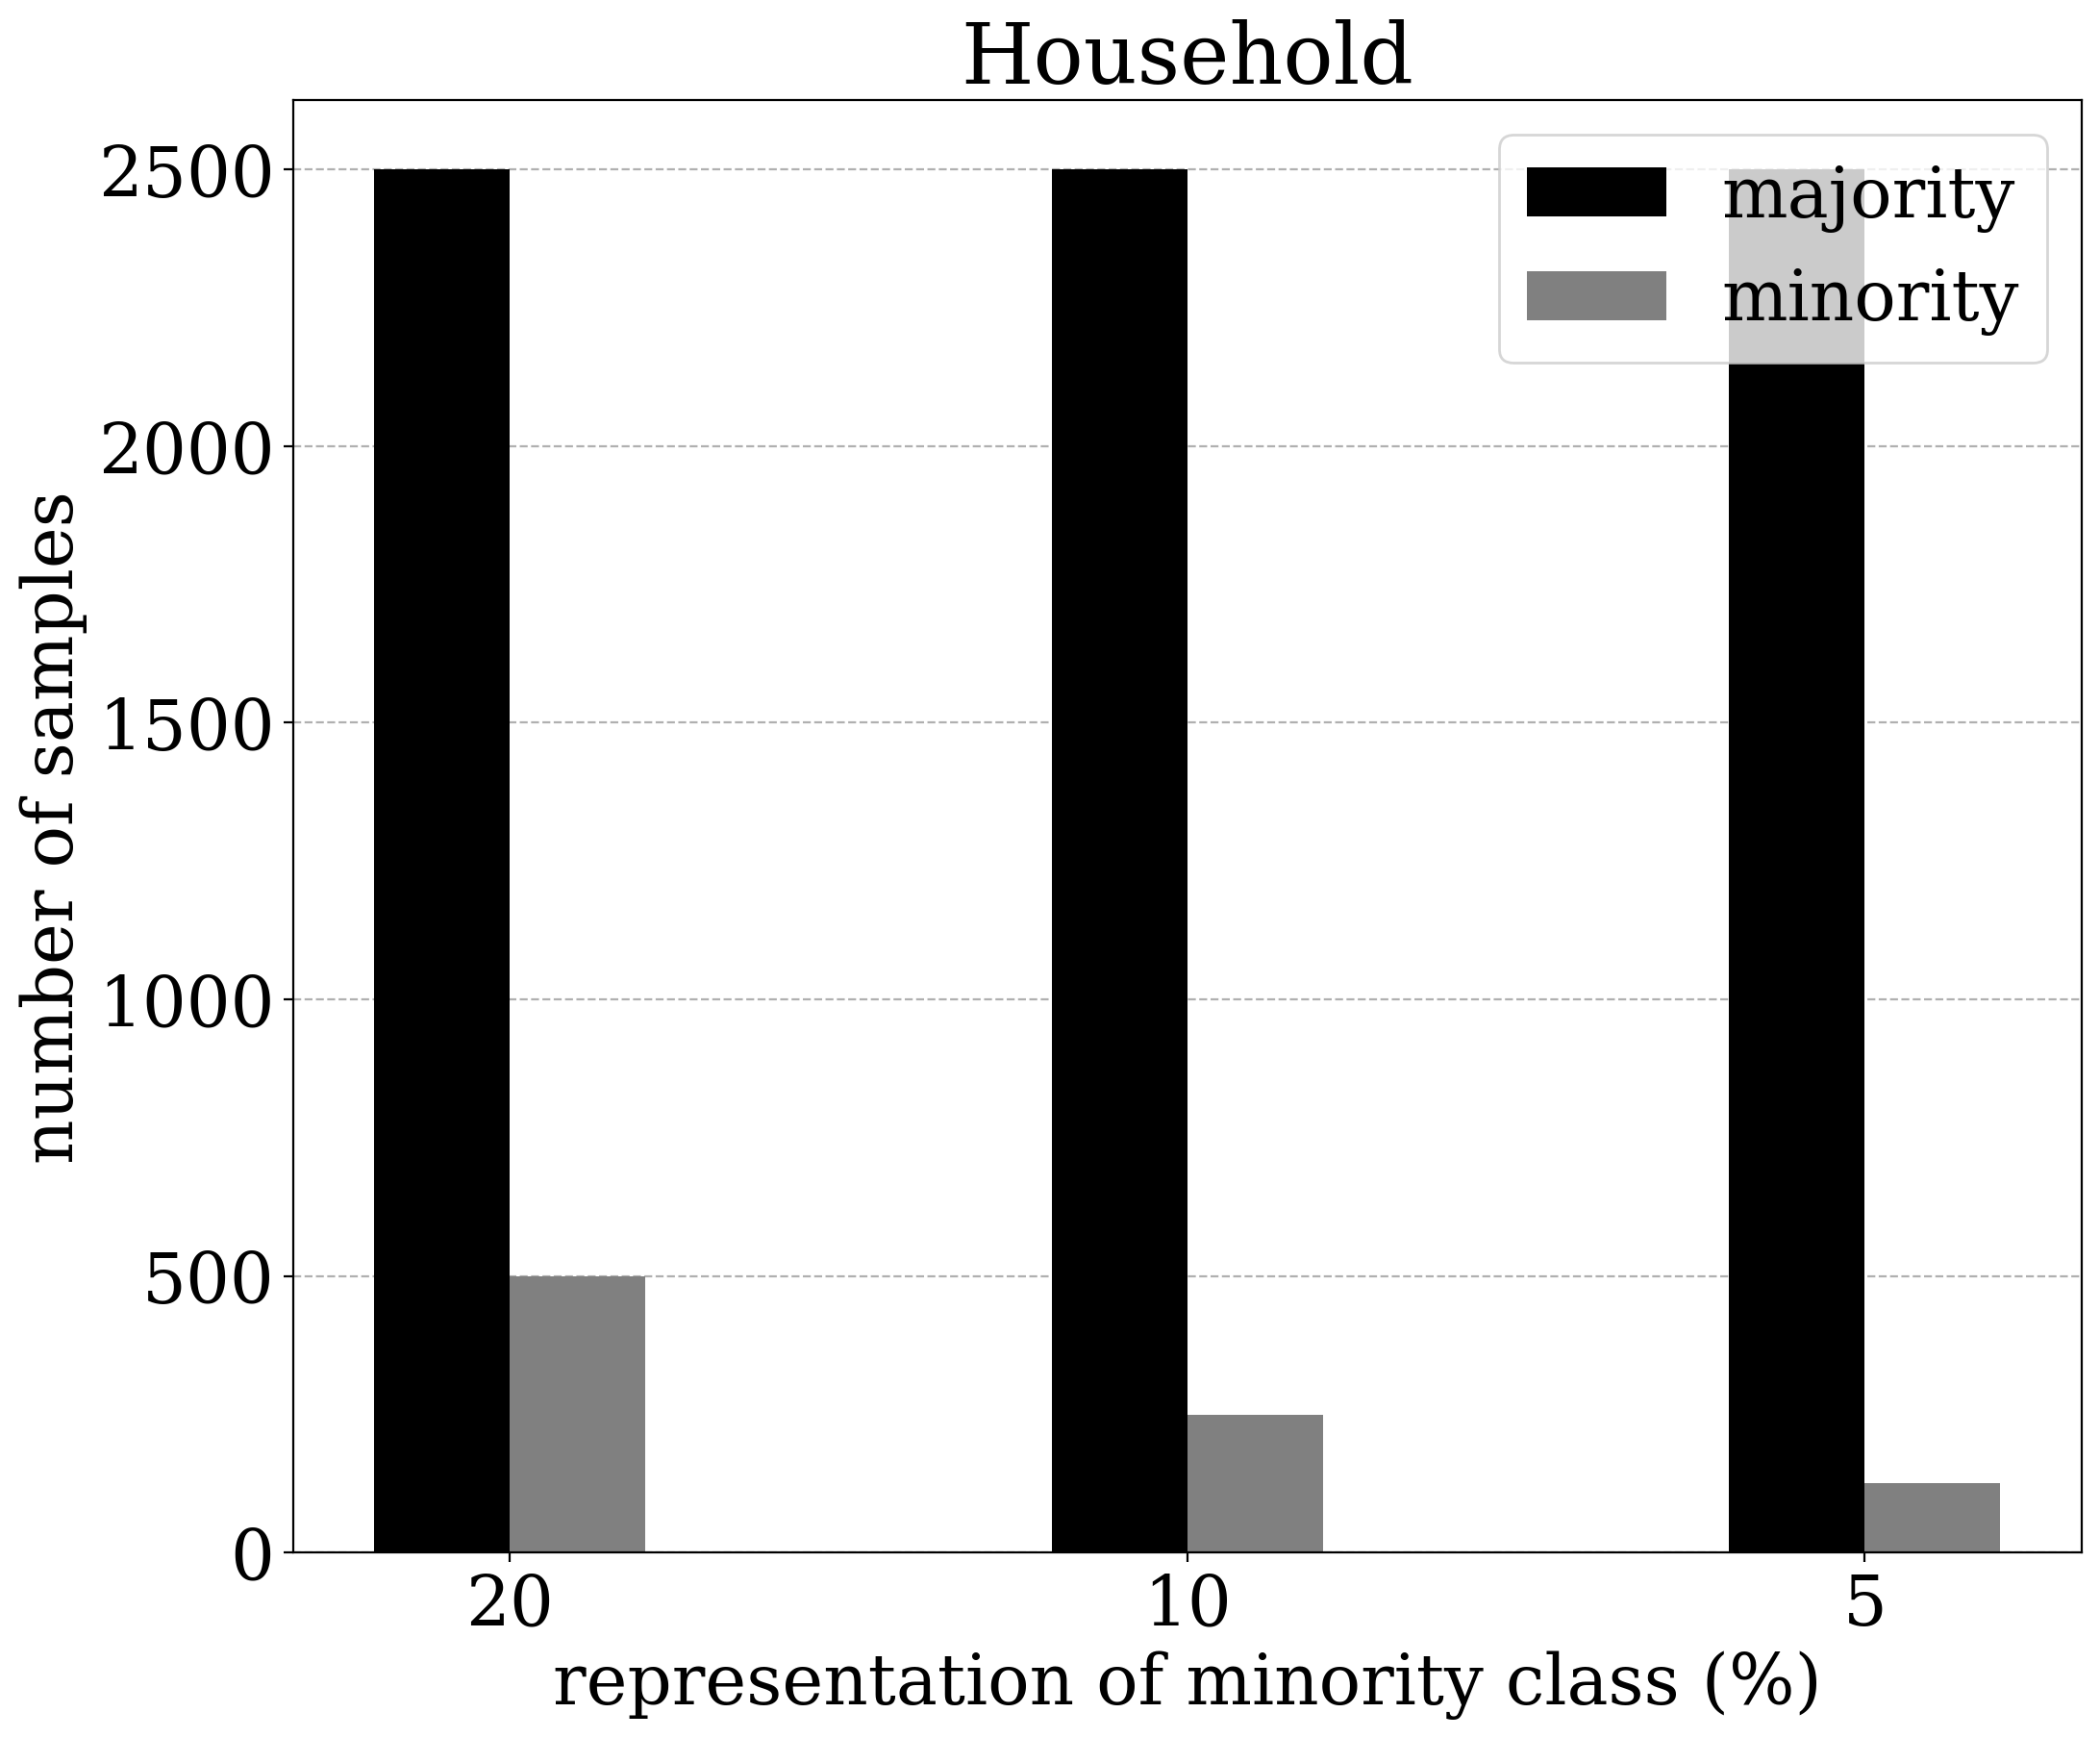
\includegraphics[width=0.45\columnwidth]{dataset/class_dist_Household_cifar100.png}
      \label{fig:dist-cifar100-household}
  }
  \caption{แสดงจำนวนตัวอย่างของกลุ่มข้อมูลส่วนมากและส่วนน้อยใน Training Set ของชุดข้อมูล \emph{Tree1}, \emph{Tree2} และ \emph{Household} ที่ร้อยละการมีอยู่ของตัวอย่างของกลุ่มข้อมูลส่วนน้อยต่าง ๆ}
  \label{fig:dist-cifar100}
\end{figure}
\FloatBarrier

\subsection{ชุดข้อมูล Benchmark}
สำหรับชุดข้อมูล Benchmark ที่ใช้ในการทดลองประกอบไปด้วย \textit{optical\_digits}, \emph{satimage}, \textit{pen\_digits} และ \emph{scene} โดยสัดส่วนจำนวนตัวอย่างของกลุ่มข้อมูลส่วนมากและส่วนน้อยใน Training ของแต่ละชุดข้อมูลแสดงดังรูปที่~\ref{fig:dist-benchmark}

\begin{figure}[h]
  \centering
   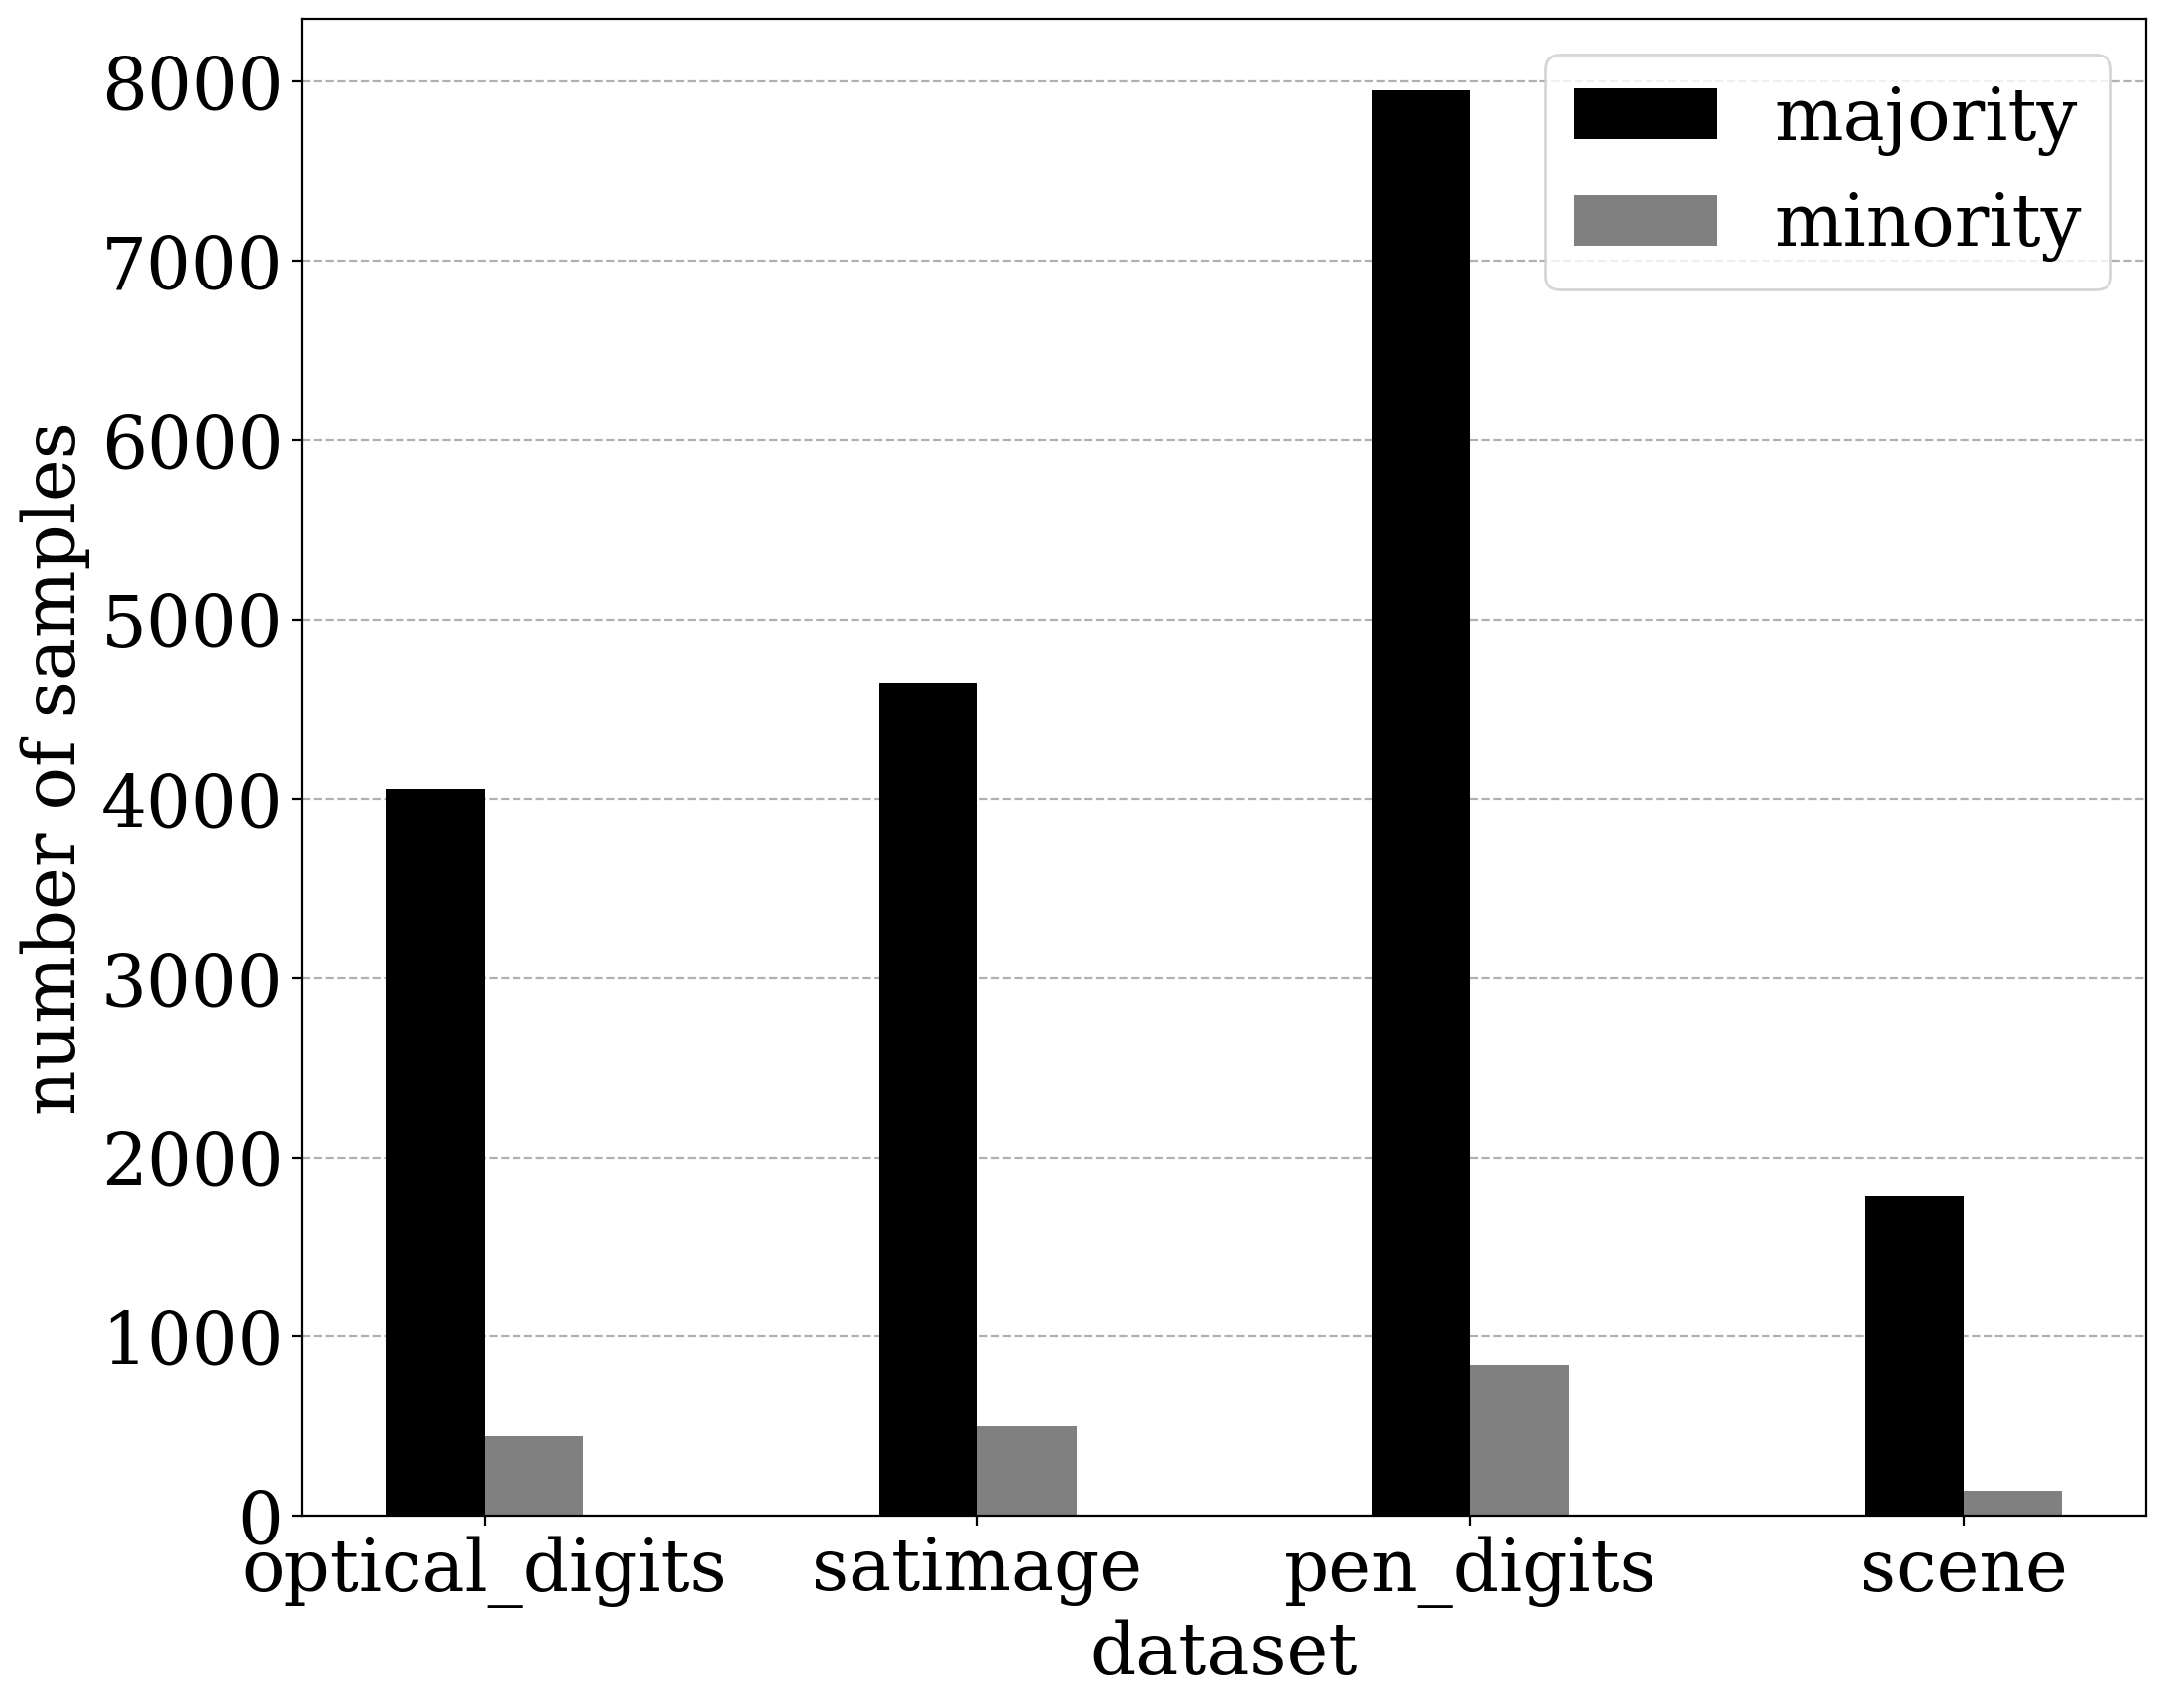
\includegraphics[width=0.45\columnwidth]{dataset/class_dist_benchmark.png}
  \caption{แสดงจำนวนตัวอย่างของกลุ่มข้อมูลส่วนมากและส่วนน้อยใน Training Set ของชุดข้อมูล \textit{optical\_digits} ($p = 9.14,~\mu = 0.09$), \emph{satimage} ($p = 9.27,~\mu = 0.09$), \textit{pen\_digits} ($p = 9.41,~\mu = 0.09$) และ \emph{scene} ($p = 12.55,~\mu = 0.07$)}
  \label{fig:dist-benchmark}
\end{figure}
\FloatBarrier

\section{การตั้งค่าเชิงเทคนิคของการทดลอง}
สำหรับสถาปัตยกรรมของแบบจำลองที่ใช้ในการทดลอง คือ แบบจำลอง ResNet~\citep{He:2016} และผู้วิจัยได้กำหนดเกณฑ์ในการหยุดกระบวนการเรียนรู้ของแบบจำลองก่อนที่จะถึงรอบสูงสุด (Early Stopping Criteria) ไว้ด้วยเพื่อความรวดเร็วในการได้มาซึ่งผลการทดลอง โดยเกณฑ์นี้จะพิจารณาที่ค่าสูญเสียของ Training Set ถ้าค่าสูญเสียไม่เปลี่ยนแปลงเป็นเวลา 10 รอบต่อเนื่อง จะทำการหยุดกระบวนการเรียนรู้ทันที สำหรับแพลตฟอร์มที่ใช้ในการพัฒนาการทดลองในงานวิจัยนี้ คือ TensorFlow~\cite{Abadi:2016}

\section{Metrics สำหรับการประเมินประสิทธิภาพของแบบจำลอง}
\subsection{F1-Score}
F1-Score เป็นค่าเฉลี่ยของ Precision และ Recall ที่ซึ่งเราสามารถพิจารณาประสิทธิภาพของแบบจำลองด้วย F1-Score แทนการพิจารณาด้วย Precision หรือ Recall โดย F1-Score สามารถคำนวณได้จากสมการที่ \ref{eq:f1-score}

\begin{equation}
  F1 = 2 * \left ( \frac{precision * recall}{precision + recall} \right )
  \label{eq:f1-score}
\end{equation}

โดยที่ Precision และ Recall สามารถคำนวณได้จากสมการที่ \ref{eq:precision} และ \ref{eq:recall} ตามลำดับ

\begin{equation}
  precision = \frac{TP}{TP + FP}
  \label{eq:precision}
\end{equation}

\begin{equation}
  recall = \frac{TP}{TP + FN}
  \label{eq:recall}
\end{equation}

โดยที่

\begin{itemize}
  \item True Positive (TP) คือ จำนวนตัวอย่างที่แบบจำลองตรวจจับได้ว่าเป็น Positive Class และตัวอย่างเหล่านั้นเป็น Positive Class
  \item True Negative (TN) คือ จำนวนตัวอย่างที่แบบจำลองตรวจจับได้ว่าเป็น Negative Class และตัวอย่างเหล่านั้นเป็น Negative Class
  \item False Positive (FP) คือ จำนวนตัวอย่างที่แบบจำลองตรวจจับได้ว่าเป็น Positive Class แต่ตัวอย่างเหล่านั้นเป็น Negative Class
  \item False Negative (FN) คือ จำนวนตัวอย่างที่แบบจำลองตรวจจับได้ว่าเป็น Negative Class แต่ตัวอย่างเหล่านั้นเป็น Positive Class
\end{itemize}

\subsection{Area Under the ROC Curve (AUC)}
AUC คือความน่าจะเป็นที่แบบจำลองจะระบุตัวอย่างของ Positive Class ว่าเป็น Positive Class และตัวอย่างของ Negative Class ว่าเป็น Negative Class 
โดยถ้าค่า AUC เข้าใกล้ 1 นั้นหมายความว่าแบบจำลองมีความสามารถในการแยก Positive Class ออกจาก Negative Class ได้เป็นอย่างดี 
ในทางเทคนิค AUC ก็คือพื้นที่ใต้กราฟของ Receiver Operating Characteristic Curve (ROC Curve) โดยความสัมพันธ์กันระหว่างค่า AUC และ ROC Curve ถูกแสดงดังรูปที่ \ref{fig:roc} 

สำหรับ ROC Curve นั้นก็คือ กราฟความสัมพันธ์ระหว่าง True Positive Rate (TPR) และ False Positive Rate (FPR) โดย TPR หรือ Recall คือ 
ความน่าจะเป็นที่แบบจำลองสามารถตรวจจับ Positive Class จากจำนวน Positive Class ทั้งหมด และ FPR คือ 
ความน่าจะเป็นที่แบบจำลองจะตรวจจับ Positive Class จากจำนวน Negative Class ทั้งหมด ทั้ง TPR และ FPR สามารถคำนวณได้จากสมการที่ \ref{eq:tpr} และ \ref{eq:fpr} ตามลำดับ

\begin{equation}
  TPR = recall = \frac{TP}{TP + FN}
  \label{eq:tpr}
\end{equation}

\begin{equation}
  FPR = \frac{FP}{FP + TN}
  \label{eq:fpr}
\end{equation}

\begin{figure}[h]
  \centering
  \subfigure[]{
      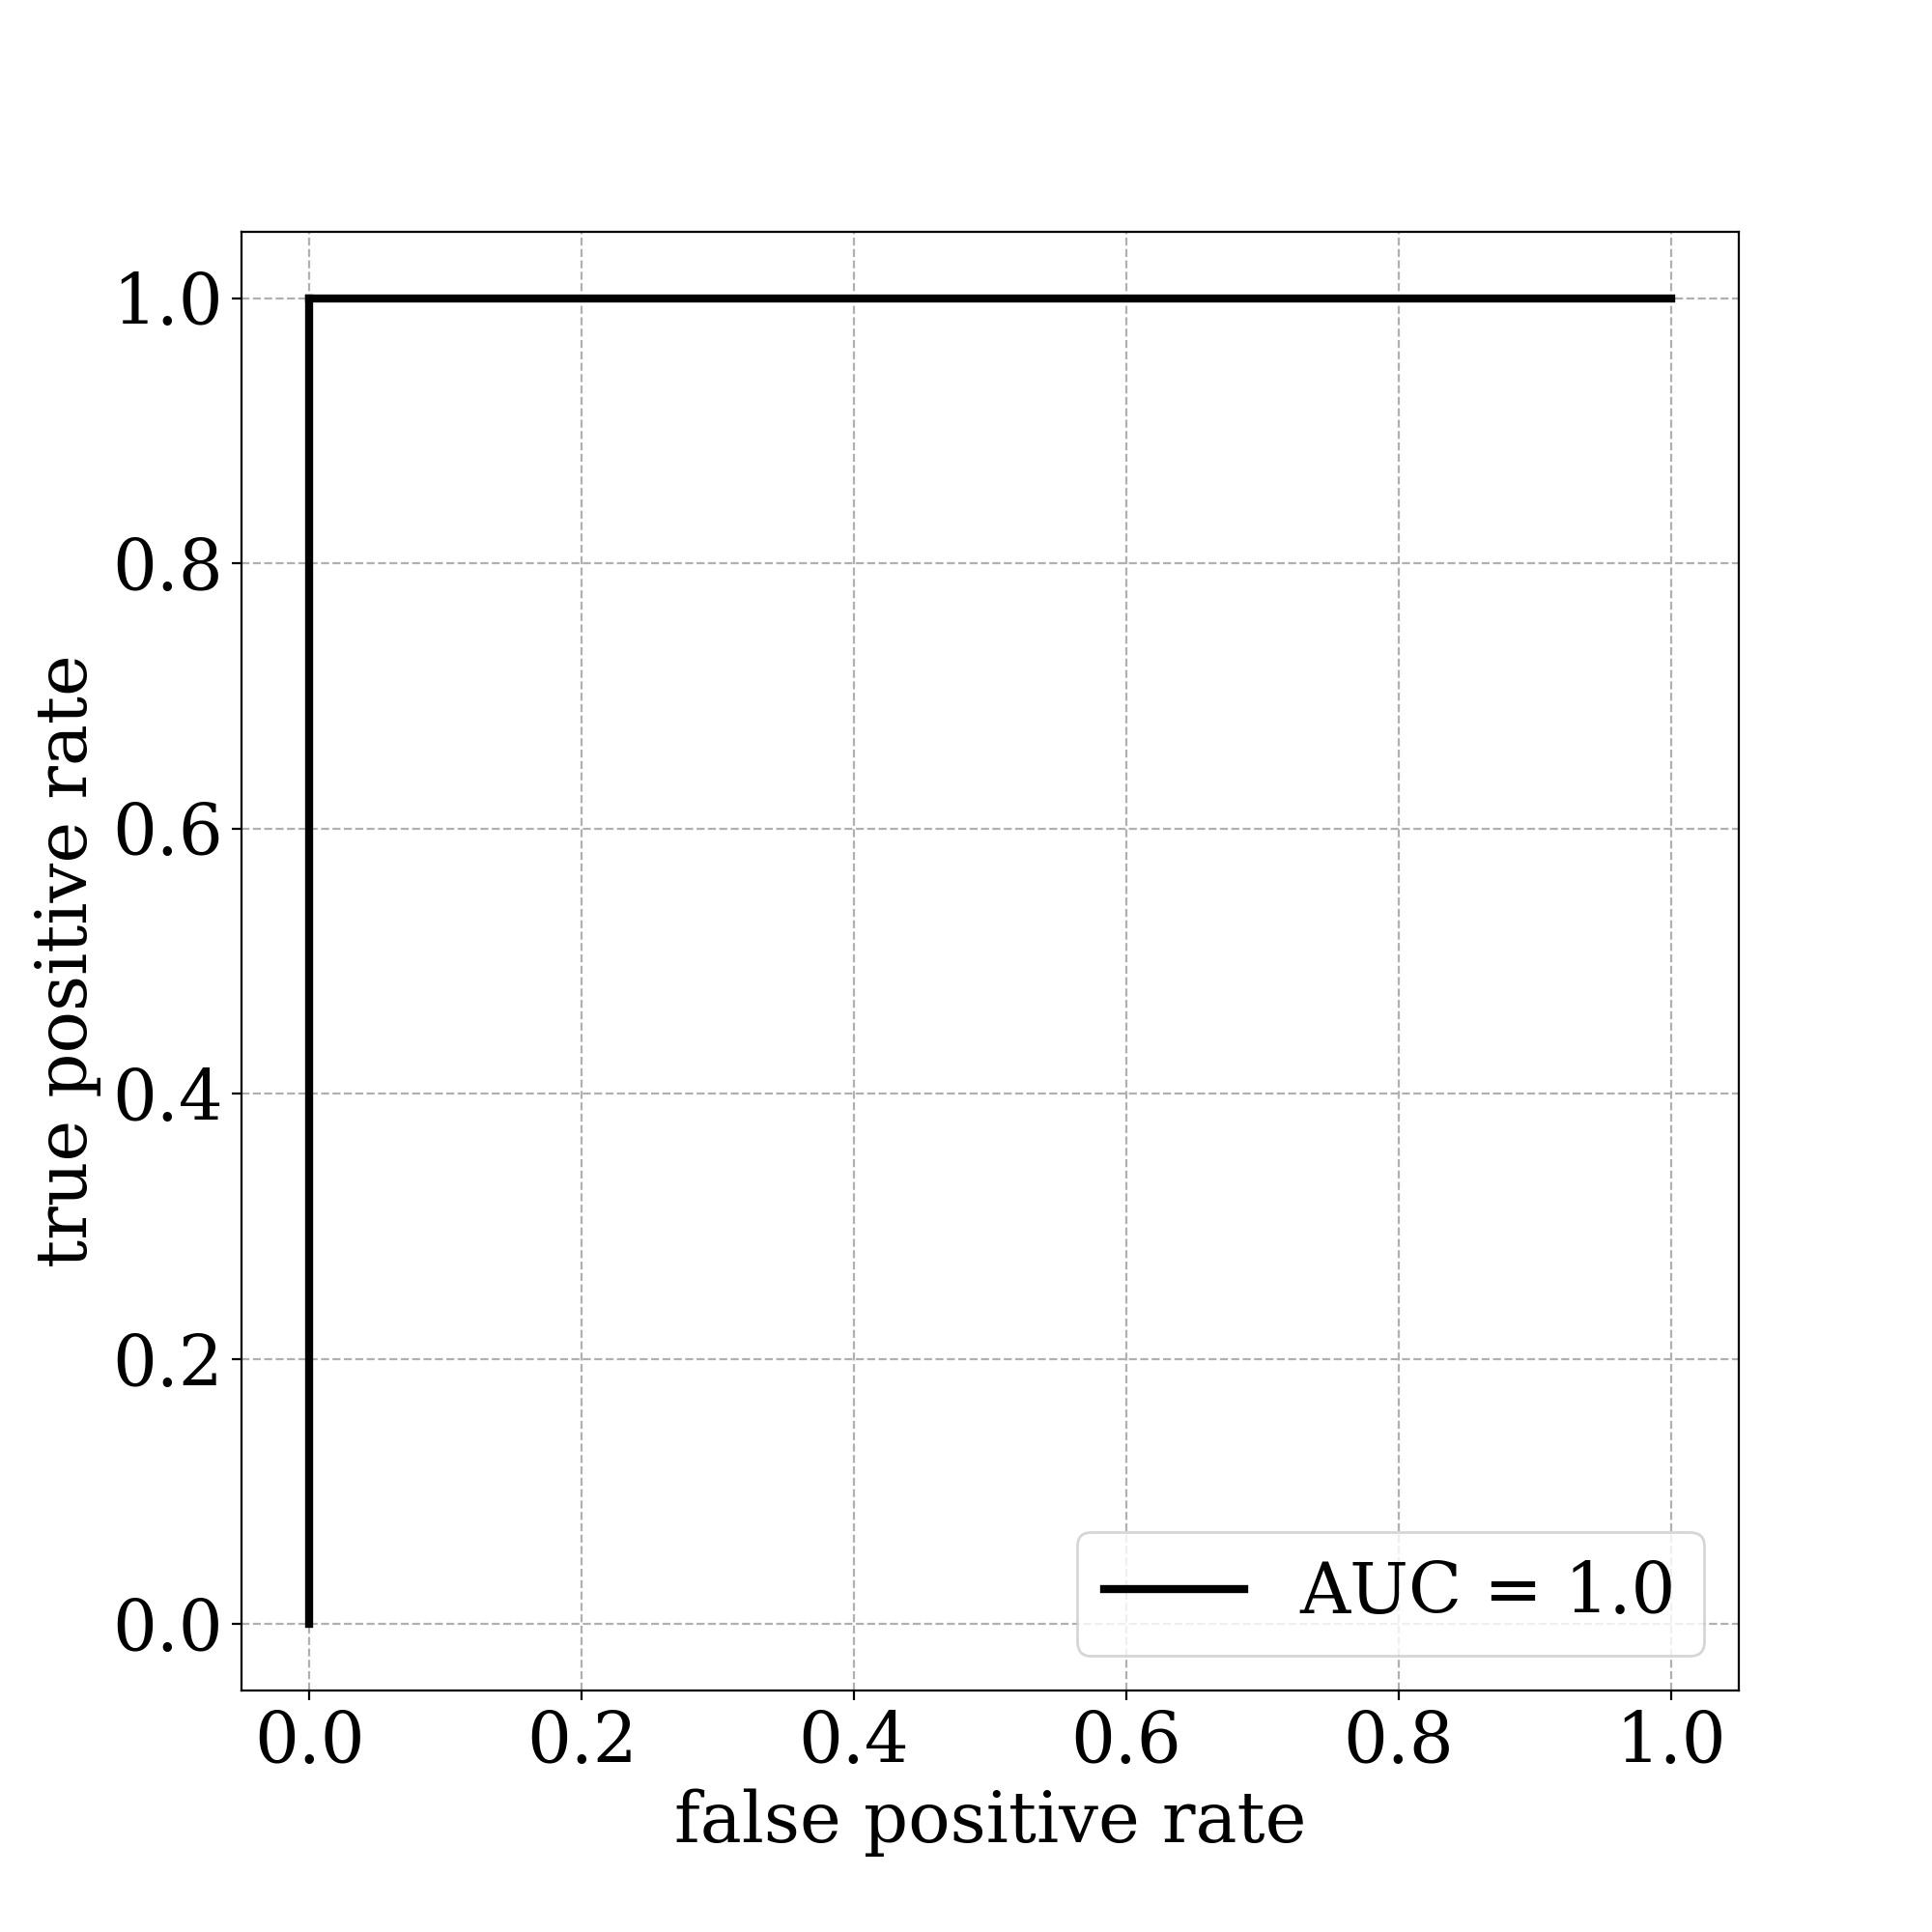
\includegraphics[width=0.45\columnwidth]{roc-1.png}
      \label{fig:roc:1}
  }
  \subfigure[]{
      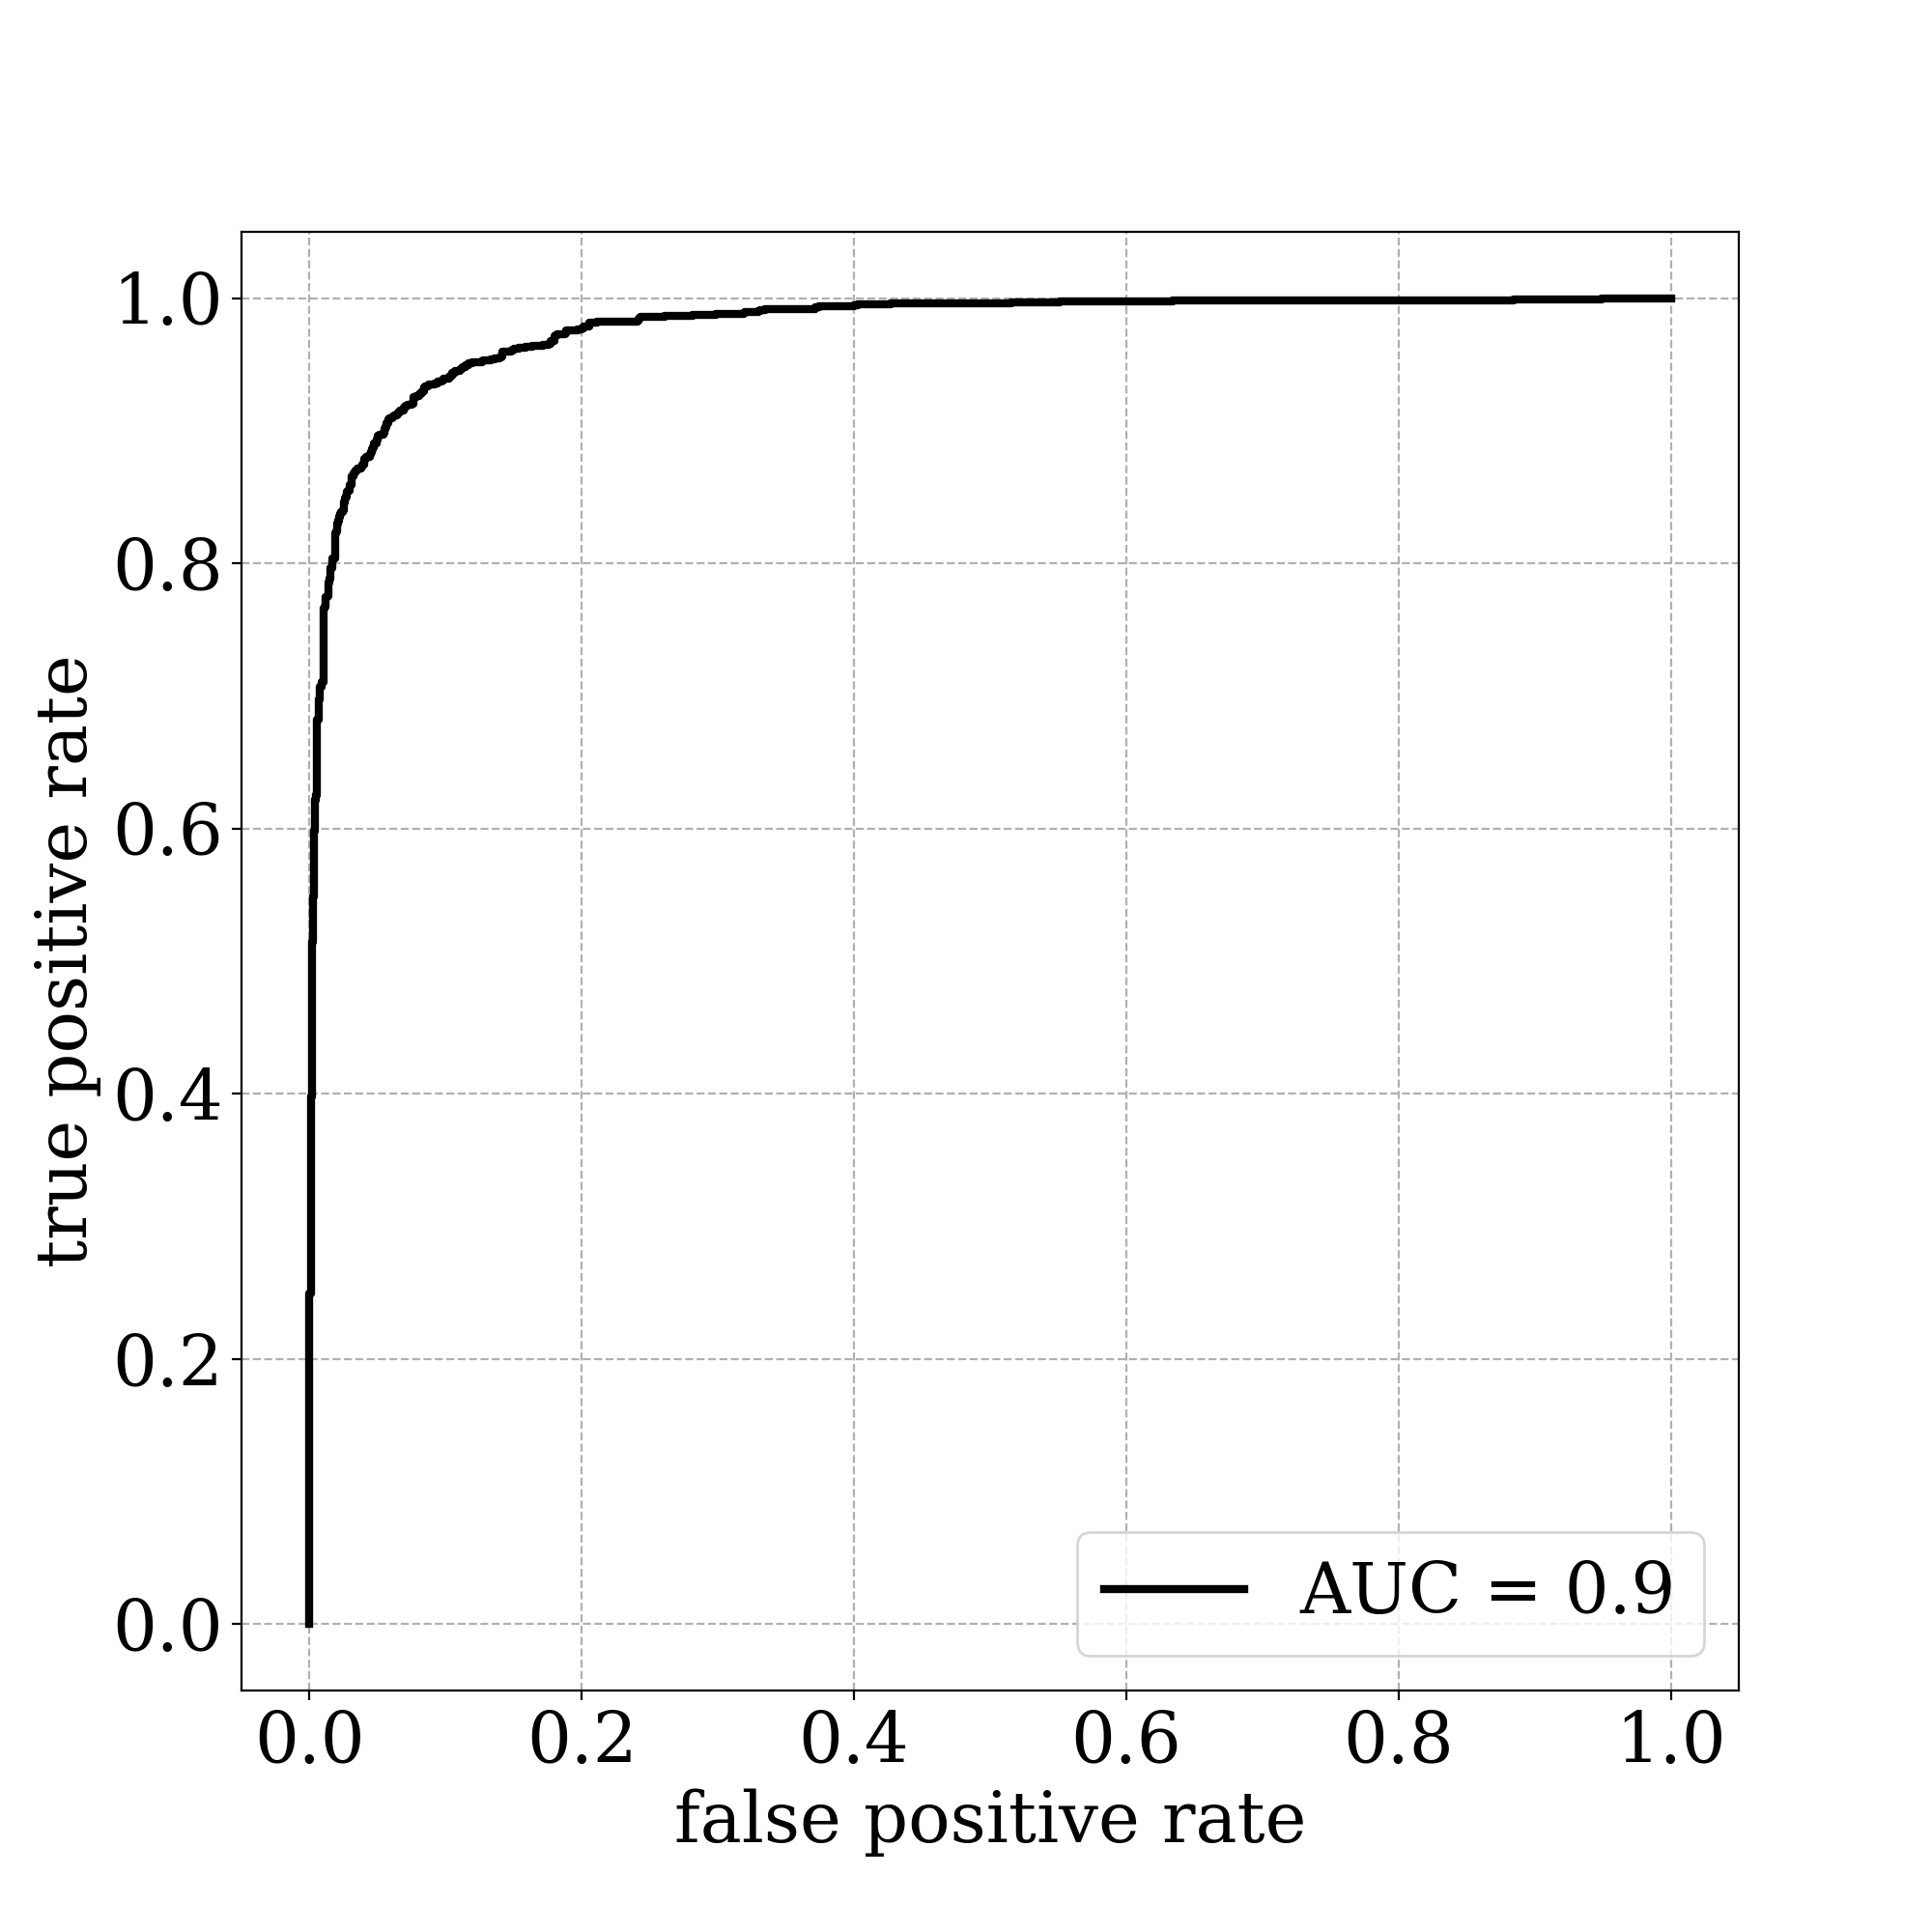
\includegraphics[width=0.45\columnwidth]{roc-2.png}
      \label{fig:roc:3}
  }
  \subfigure[]{
    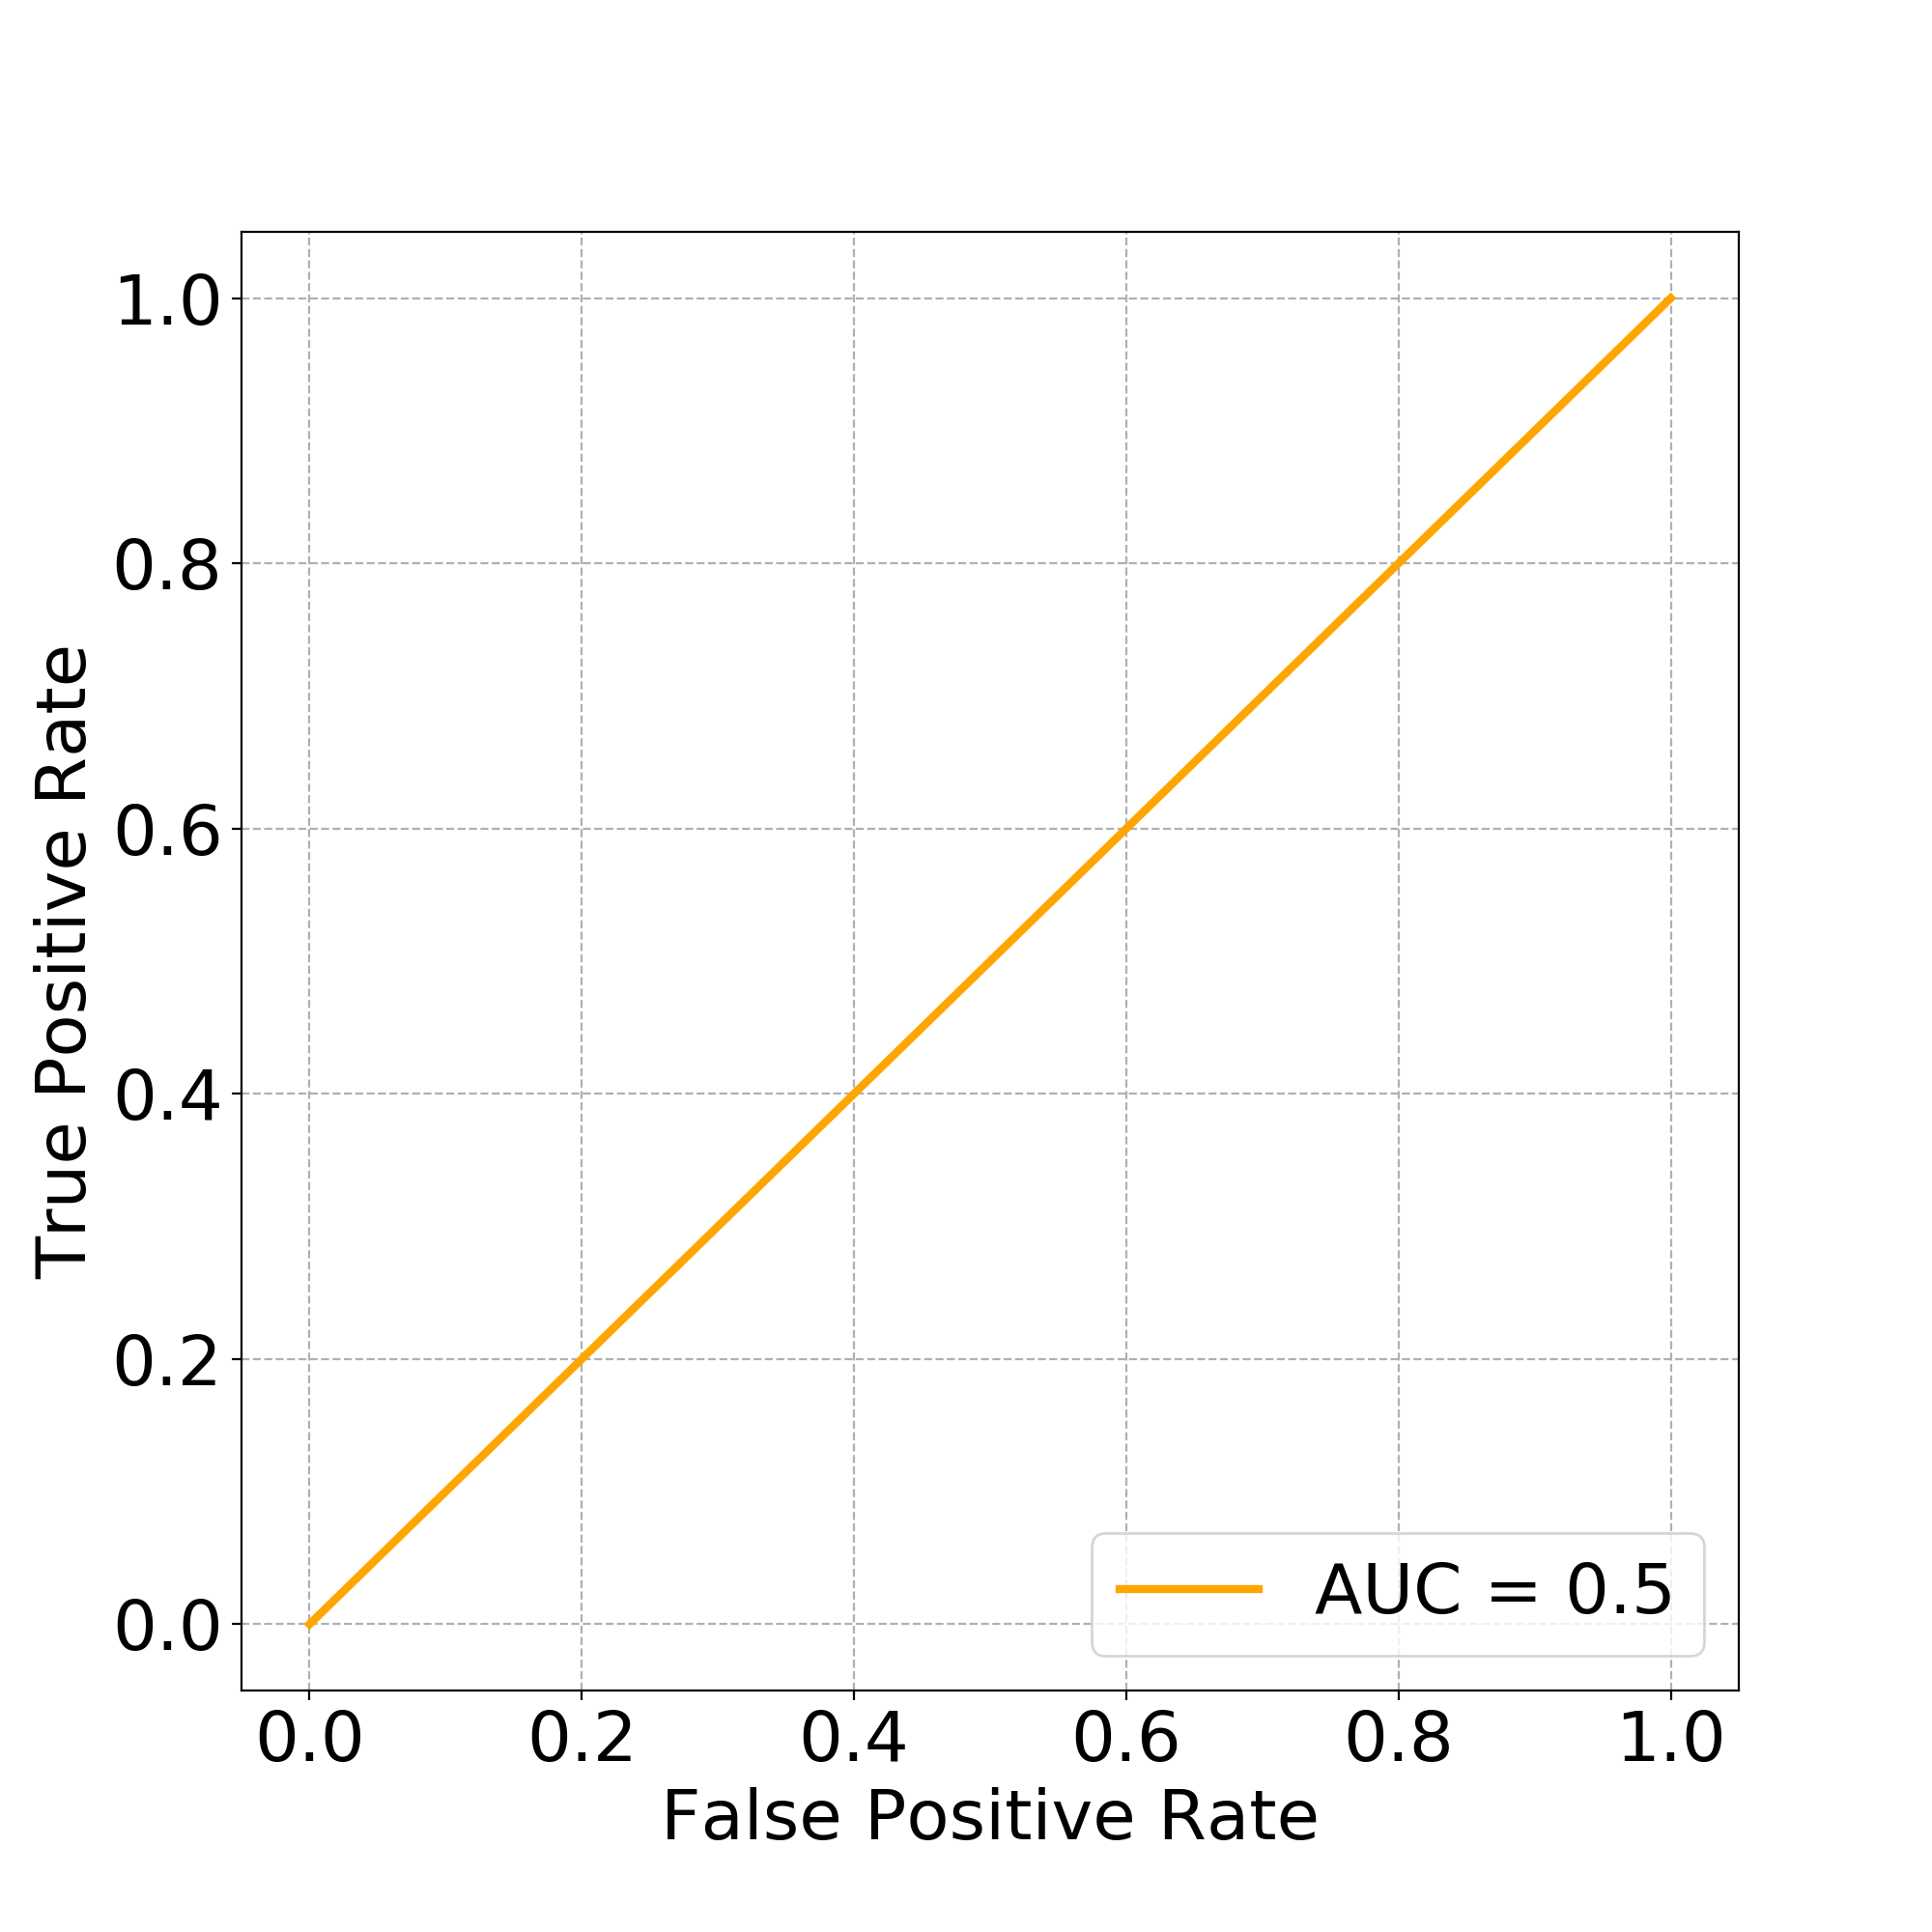
\includegraphics[width=0.45\columnwidth]{roc-3.png}
    \label{fig:roc:3}
  }
  \subfigure[]{
    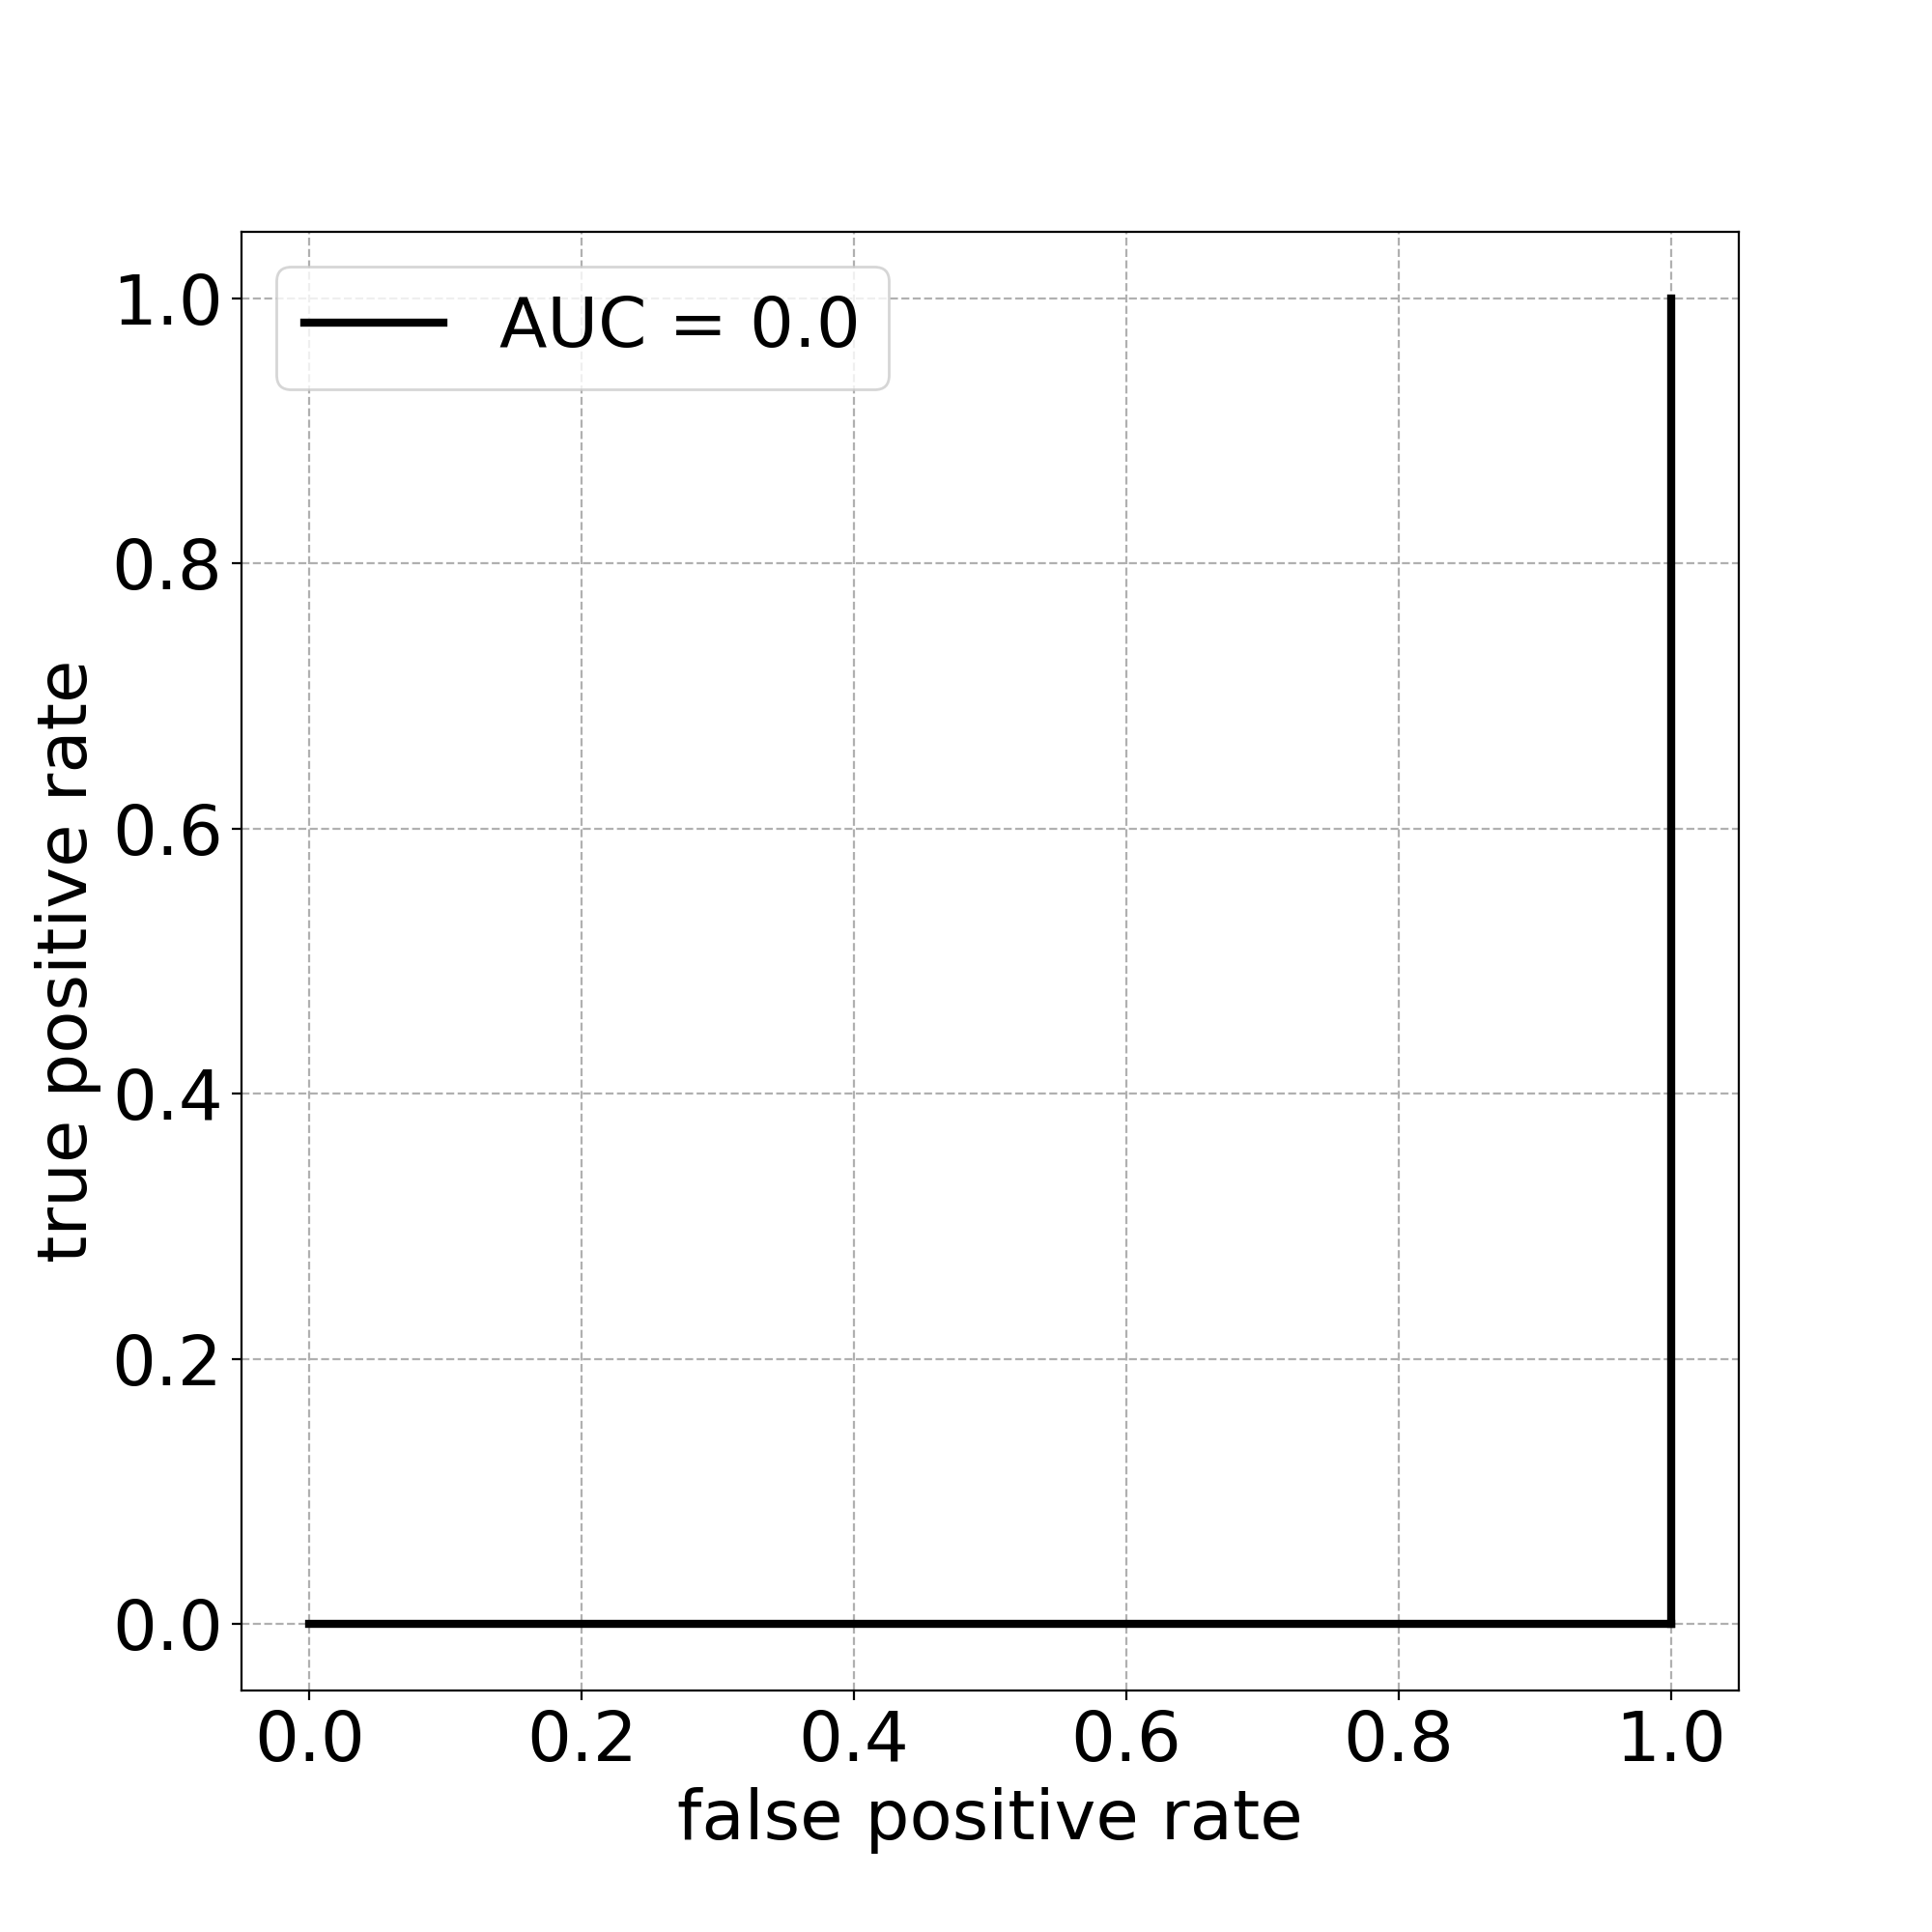
\includegraphics[width=0.45\columnwidth]{roc-4.png}
    \label{fig:roc:3}
  }
  \caption{ตัวอย่างกราฟ ROC Curve แบบต่าง ๆ}
  \label{fig:roc}
\end{figure}
\FloatBarrier

\section{ผลการทดลอง}
\subsection{ผลการทดลองกับชุดข้อมูลดัดแปลง}

รูปที่~\ref{fig:result-cifar100} แสดงผลการทดลองของแต่ละชุดข้อมูล โดยจากผลการทดลองสามารถสรุปได้ว่าฟังก์ชันสูญเสียแบบ Hybrid มีประสิทธิภาพเหนือกว่าฟังก์ชันสูญเสียอื่น ๆ อย่างสิ้นเชิง

\begin{figure}[h]
  \centering
  \subfigure[]{
      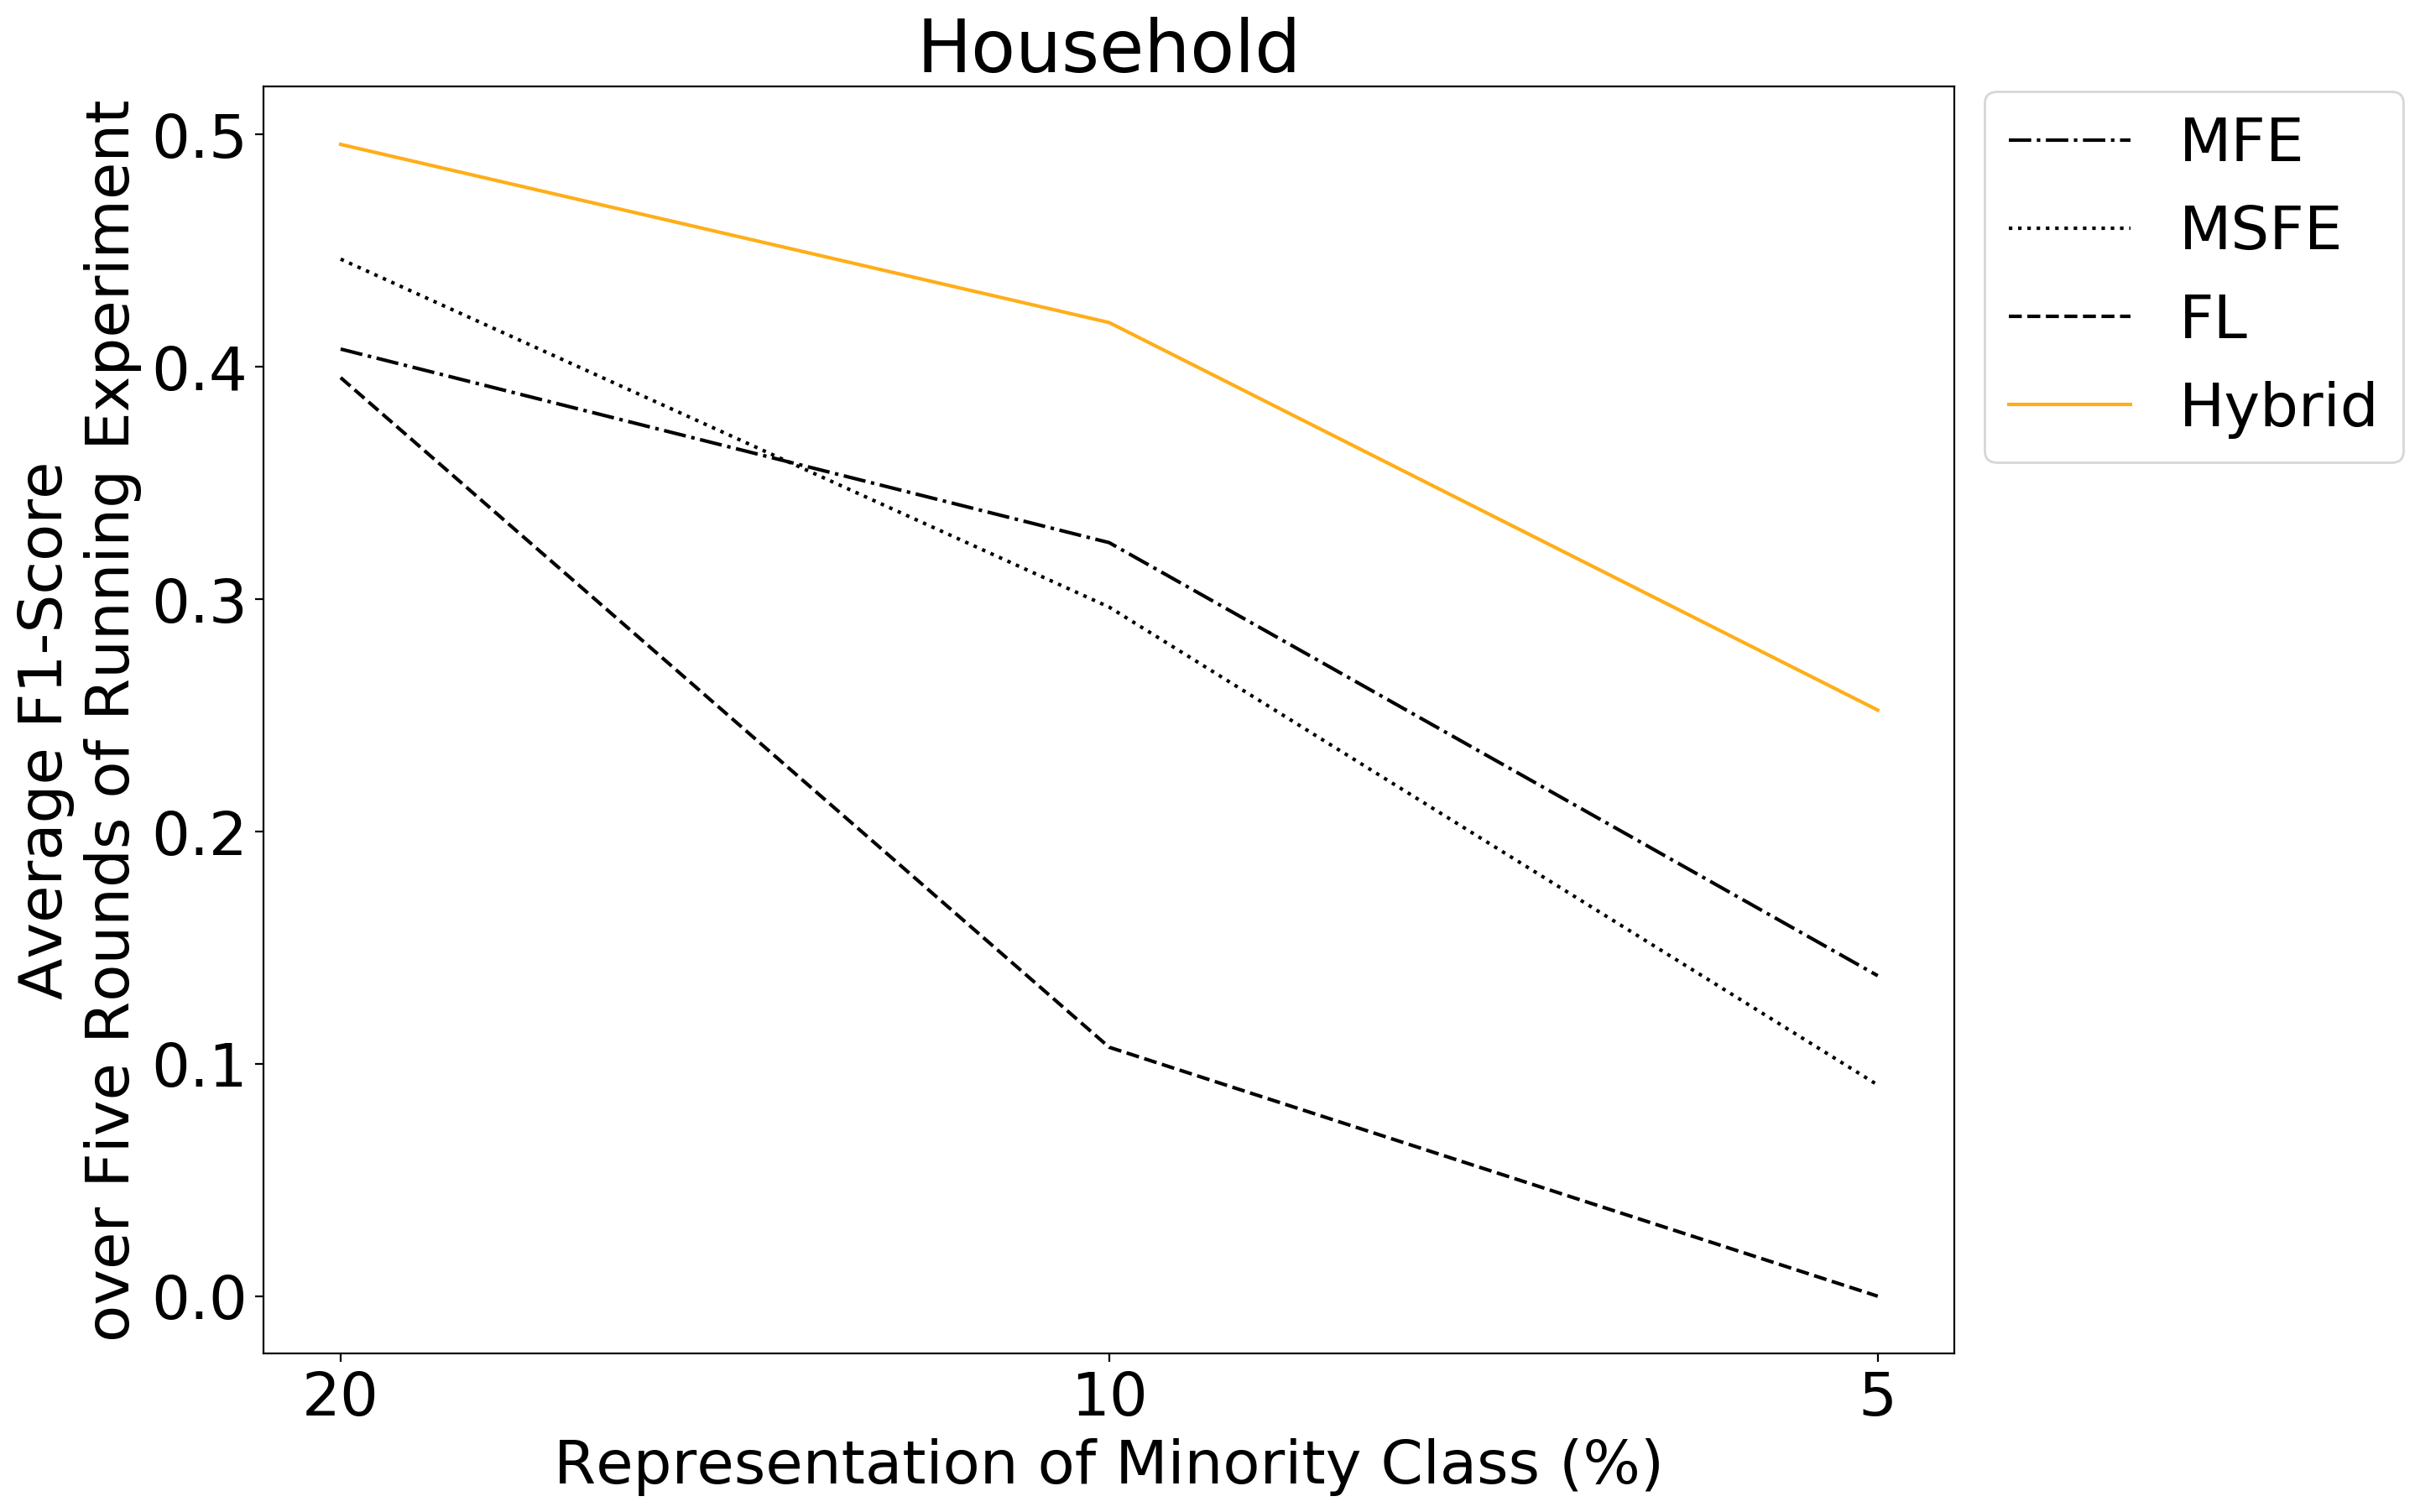
\includegraphics[width=0.9\columnwidth]{results/Household_cifar100.png}
      \label{fig:result-cifar100-household}
  }
  \subfigure[]{
      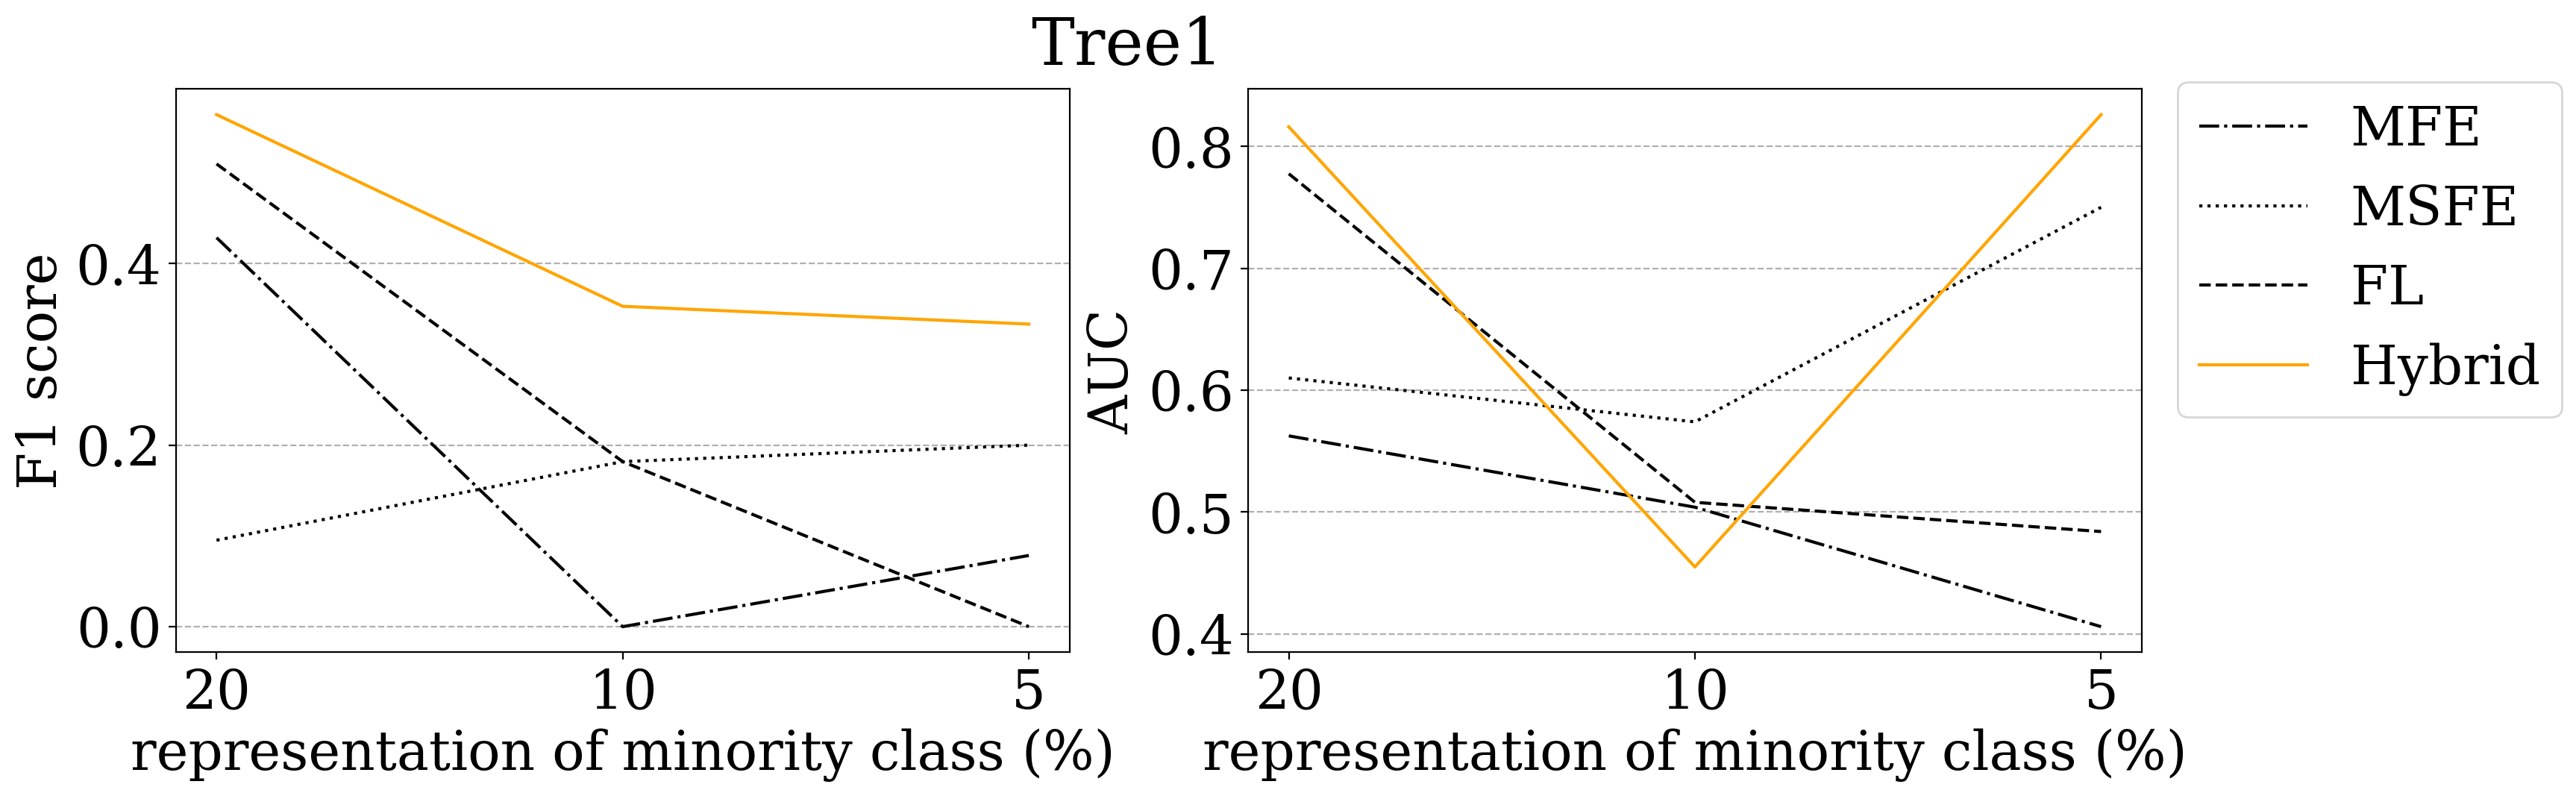
\includegraphics[width=0.9\columnwidth]{results/Tree1_cifar100.png}
      \label{fig:result-cifar100-tree1}
  }
  \subfigure[]{
    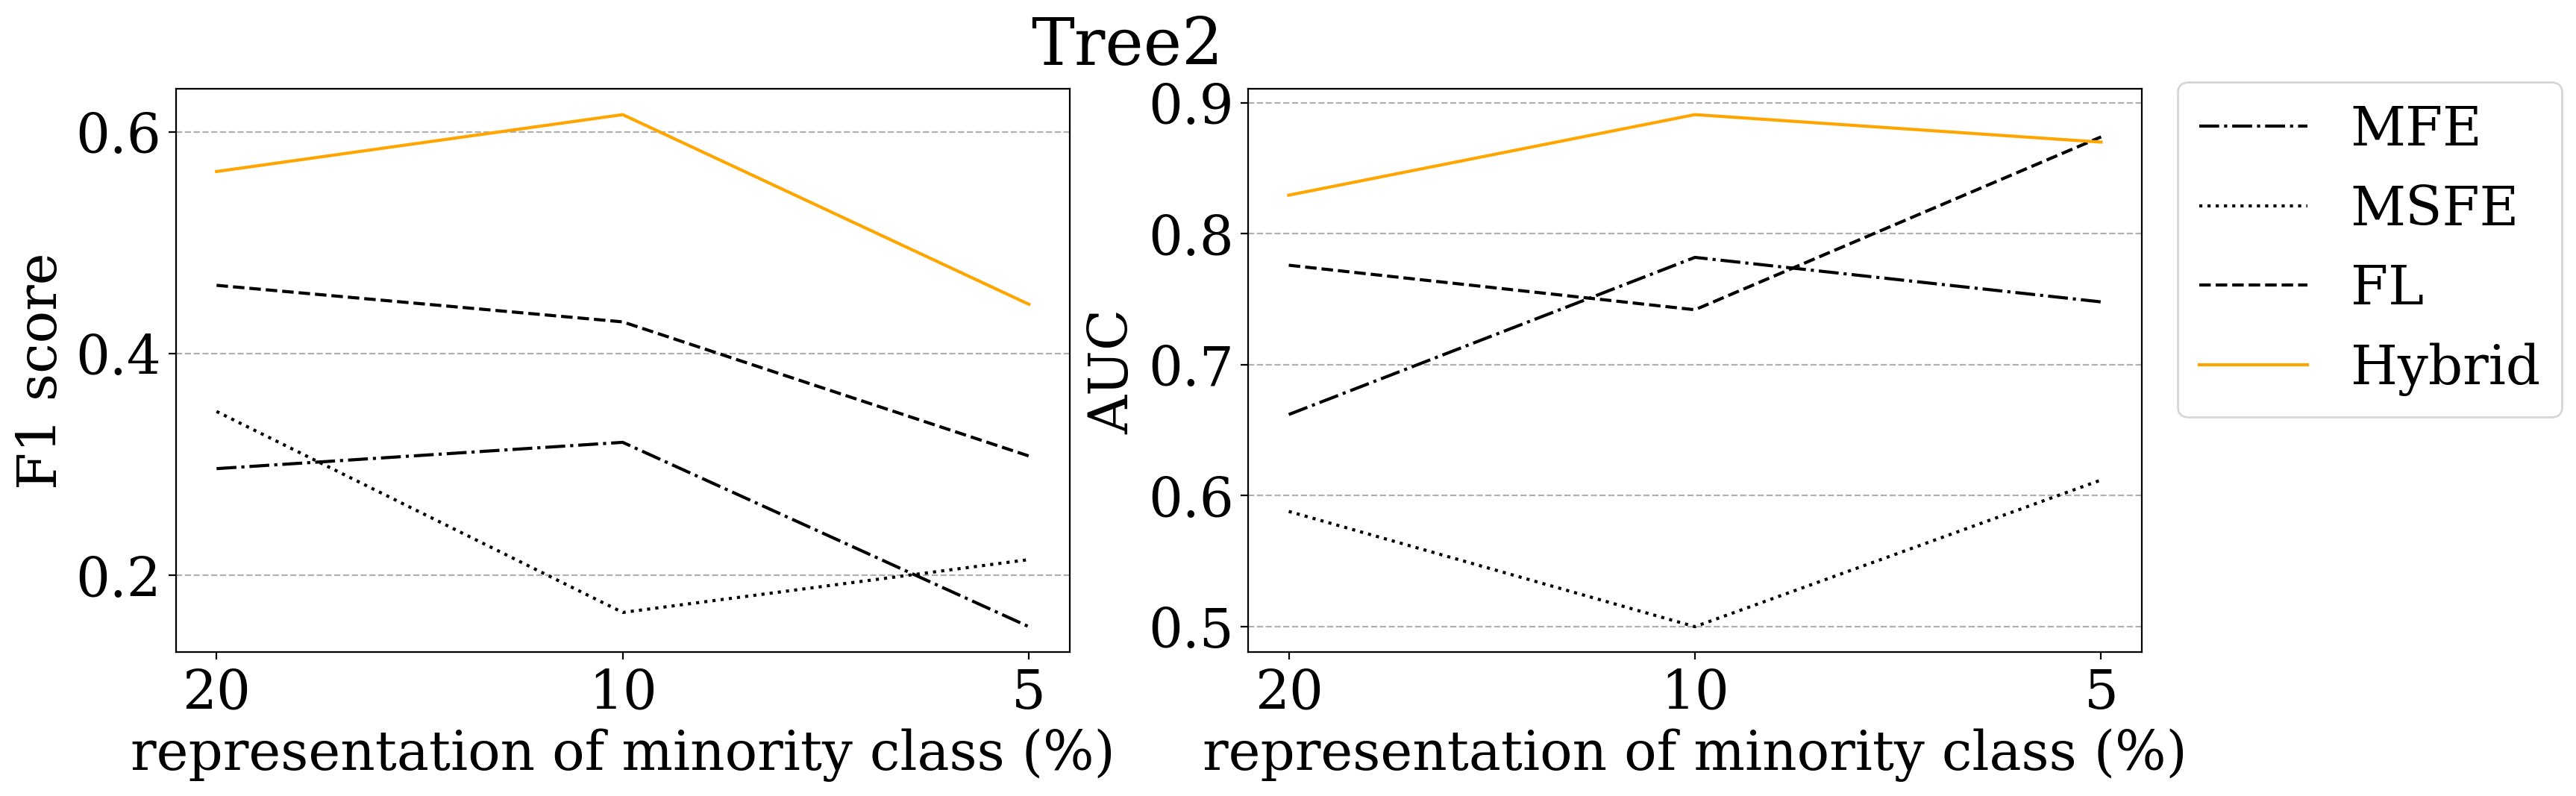
\includegraphics[width=0.9\columnwidth]{results/Tree2_cifar100.png}
    \label{fig:result-cifar100-tree2}
  }
  \caption{ประสิทธิภาพของแต่ละฟังก์ชันสูญเสีย เมื่อทดสอบกับชุดข้อมูลที่มีอัตราจำนวนตัวอย่างของกลุ่มข้อมูลส่วนน้อยที่แตกต่างกัน}
  \label{fig:result-cifar100}
\end{figure}
\FloatBarrier

ผู้วิจัยได้สำรวจ Learning Curve ของแต่ละฟังก์ชันสูญเสียดังรูปที่~\ref{fig:result-loss} จาก Learning Curve ของฟังก์ชันสูญเสีย Hybrid จะเห็นได้ว่าค่าสูญเสียนั้นค่อนข้างเหวี่ยงในบางชุดข้อมูล ซึ่ง Learning Curve ของฟังก์ชันสูญเสีย MSFE ก็มีลักษณะเช่นเดียวกัน อย่างไรก็ตามฟังก์ชันสูญเสีย Hybrid ยังคงมีประสิทธิภาพเชิงความแม่นยำที่ดีกว่าฟังก์ชันอื่น ๆ

จากรูปที่~\ref{fig:result-loss} เนื่องจากในการทดลองมีการใช้ Early Stopping Criteria ด้วย จำนวนรอบในการเรียนรู้จึงต่างกัน และสามารถสรุปได้ว่าจำนวนรอบที่ใช้ในการเรียนรู้ของแต่ละฟังก์ชันสูญเสียมีความใกล้เคียงกัน 

\begin{figure}[h]
  \centering
  \subfigure[]{
      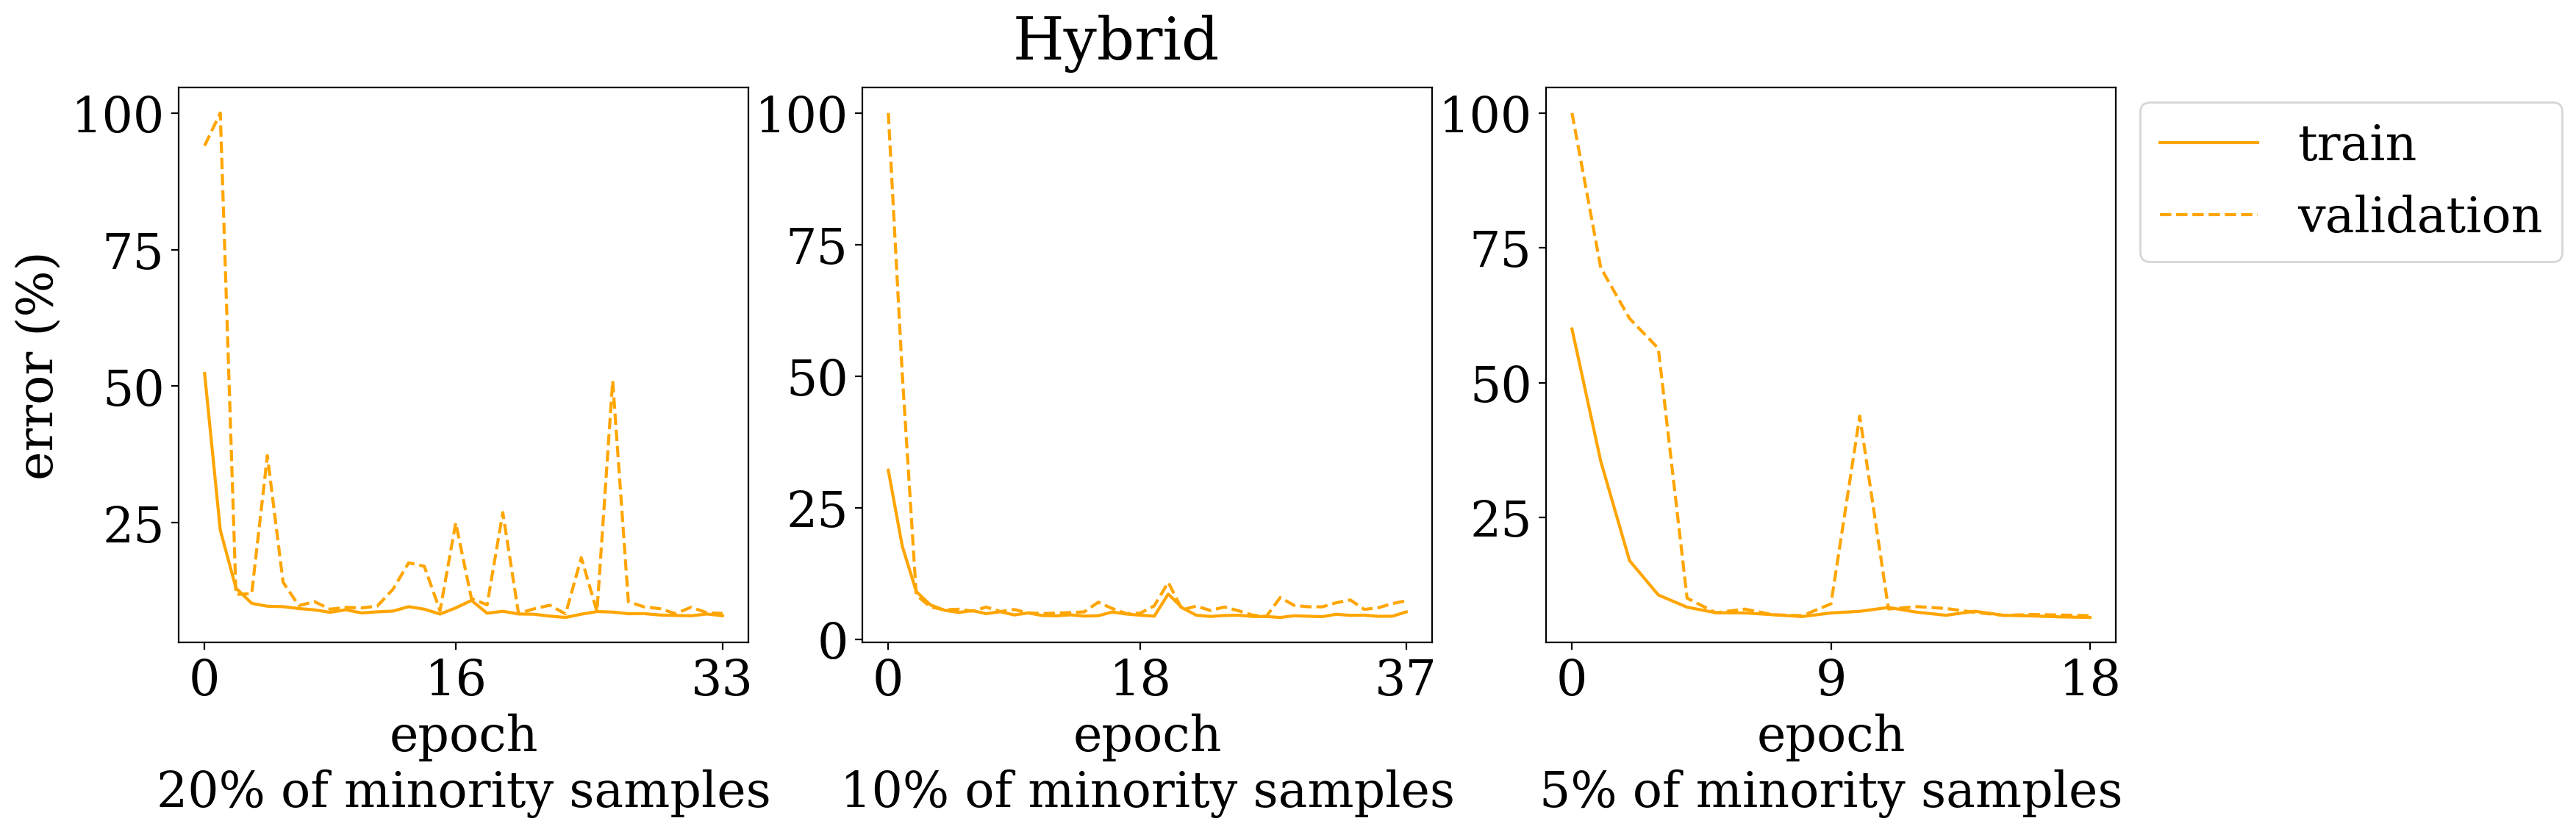
\includegraphics[width=0.95\columnwidth]{results/Household_cifar100_Balanced-Hybrid.png}
      \label{fig:result-loss-hybrid}
  }
  \subfigure[]{
      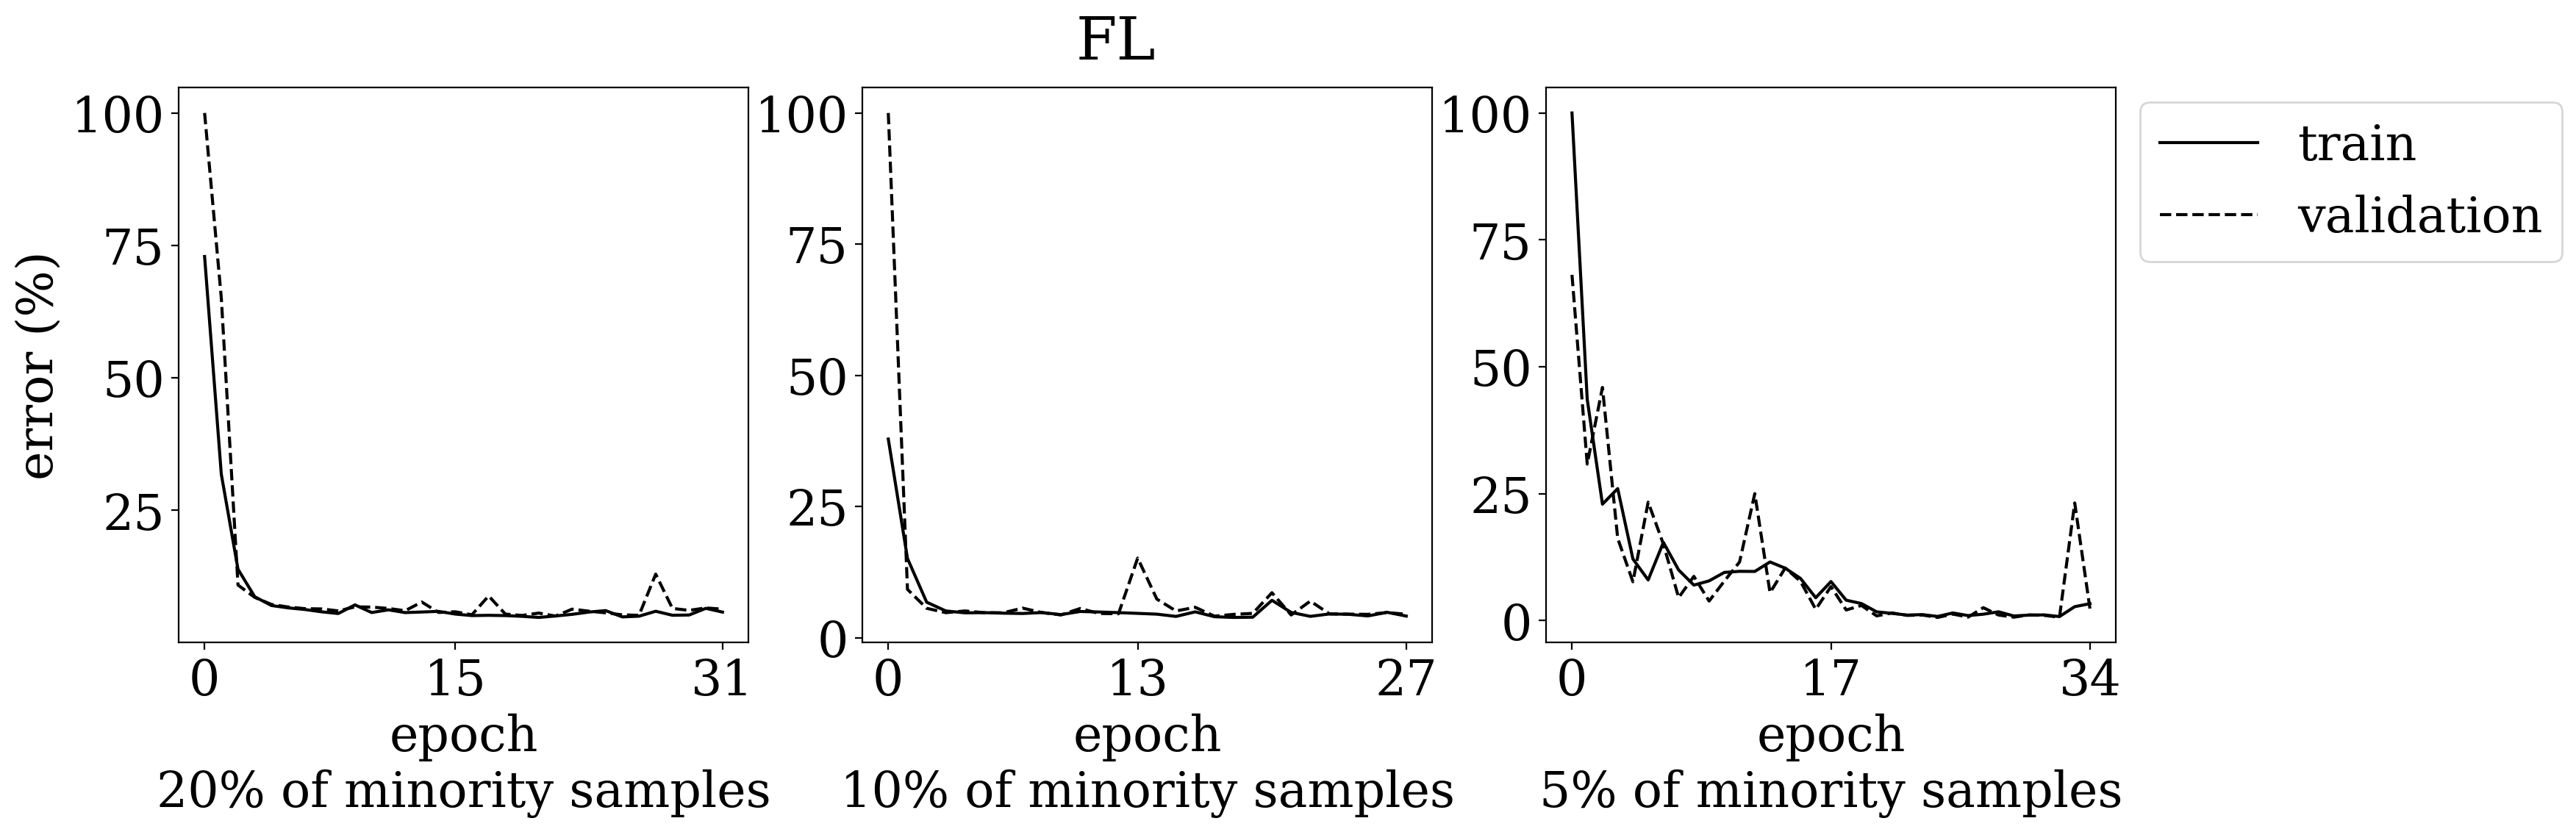
\includegraphics[width=0.95\columnwidth]{results/Household_cifar100_Balanced-FL.png}
      \label{fig:result-loss-fl}
  }
  \subfigure[]{
    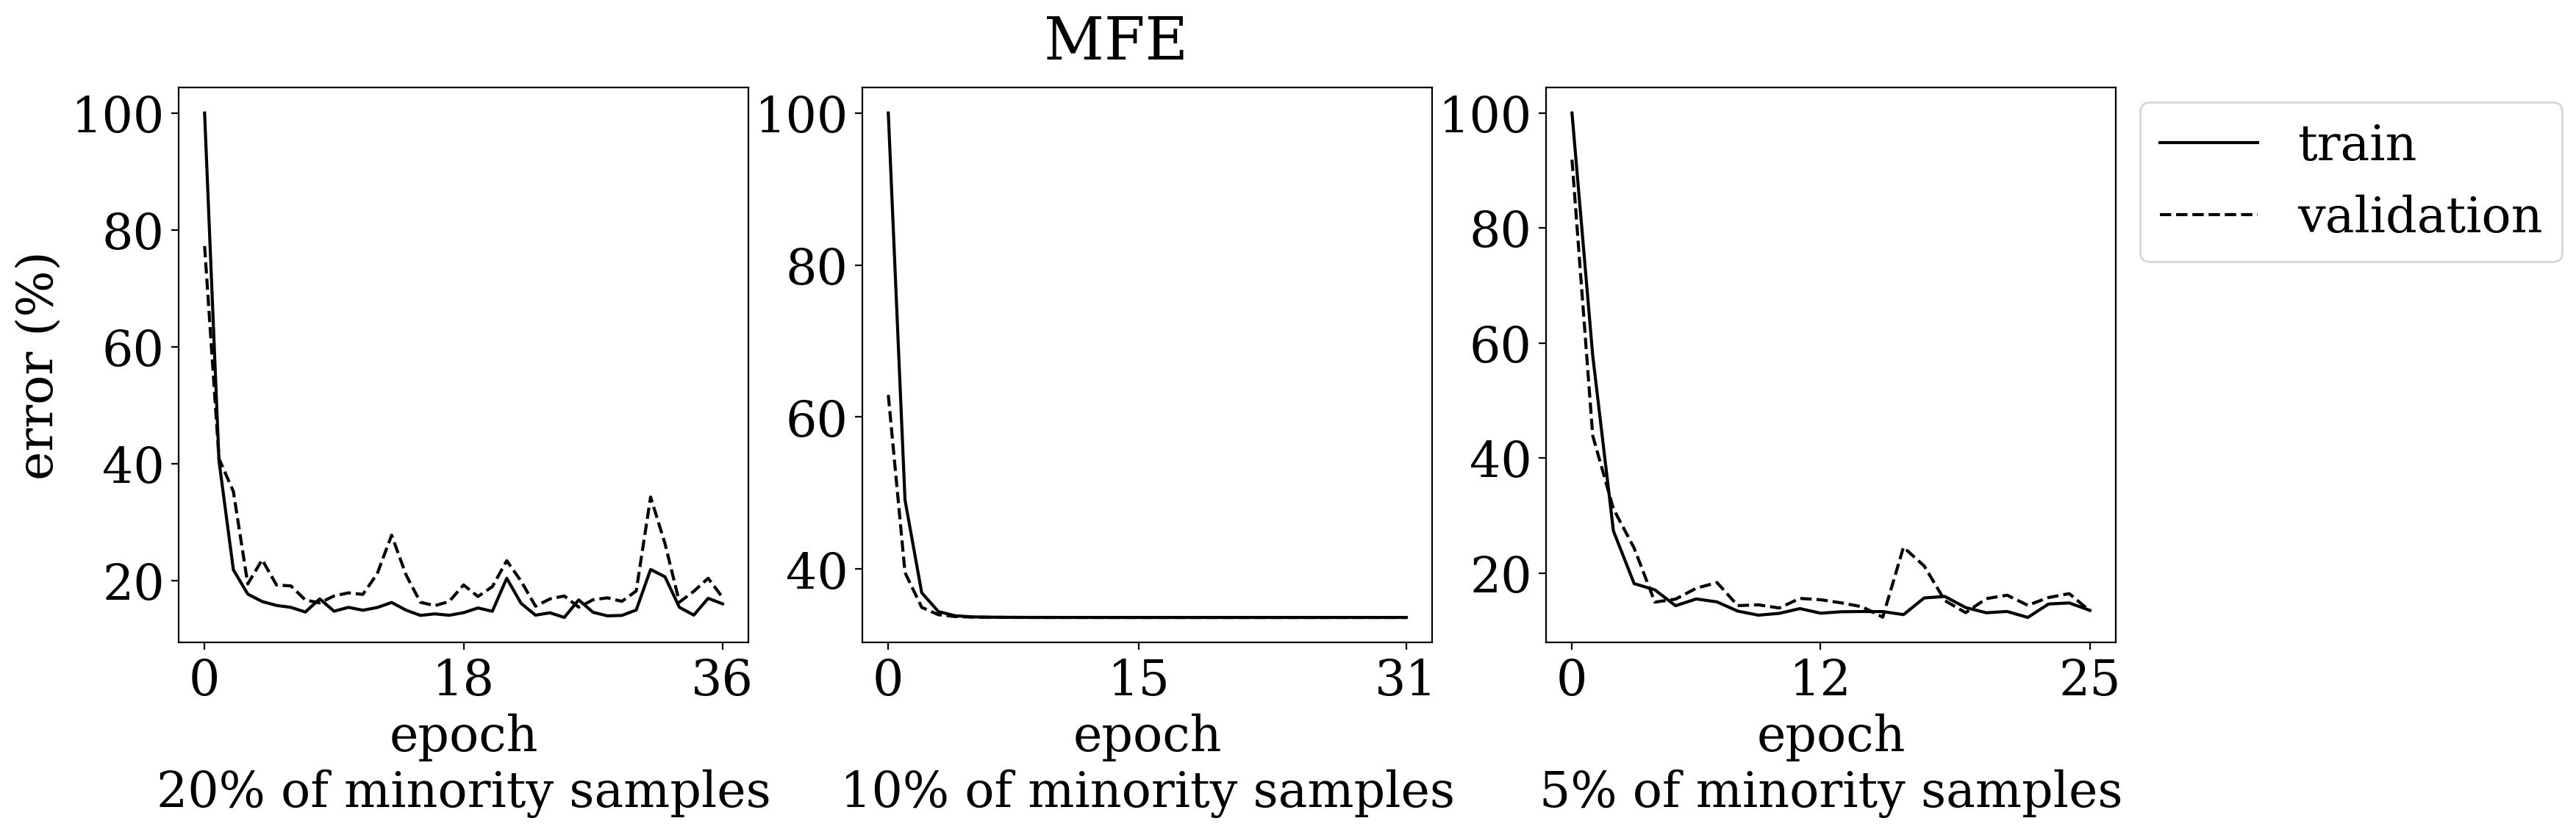
\includegraphics[width=0.95\columnwidth]{results/Household_cifar100_MFE.png}
    \label{fig:result-loss-mfe}
  }
  \subfigure[]{
    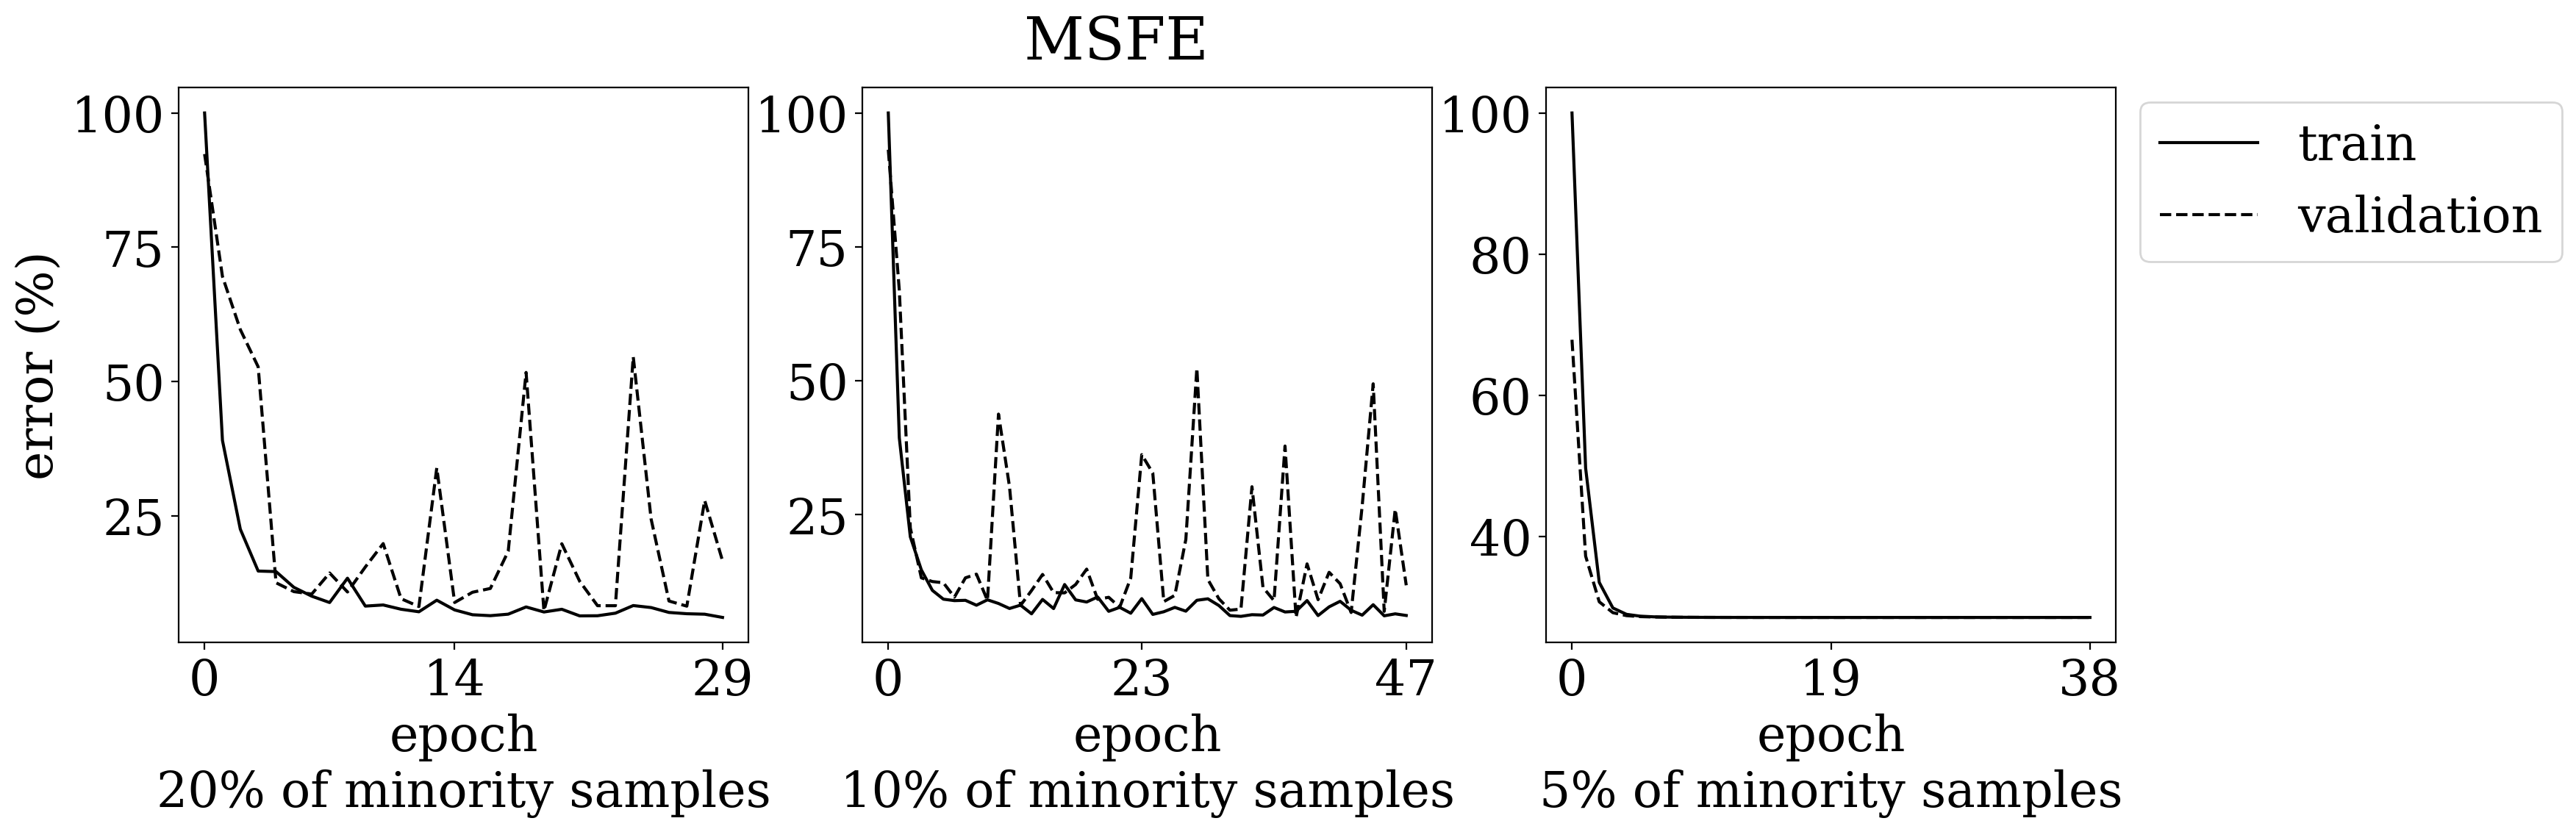
\includegraphics[width=0.95\columnwidth]{results/Household_cifar100_MSFE.png}
    \label{fig:result-loss-msfe}
  }
  \caption{ค่าสูญเสียในแต่ละรอบของการเรียนรู้ของแบบจำลอง เมื่อเรียนรู้จากชุดข้อมูล Household ที่ร้อยละการมีอยู่ของตัวอย่างของกลุ่มข้อมูลส่วนน้อยต่าง ๆ}
  \label{fig:result-loss}
\end{figure}

\subsection{ผลการทดลองกับชุดข้อมูล Benchmark}